% Chapter Template

\chapter{Plan Production and Management} % Main chapter title

\label{chapter:plan_management} % Change X to a consecutive number; for referencing this chapter elsewhere, use \ref{ChapterX}

\lhead{Chapter 4. \emph{Plan Production and Management}} % Change X to a consecutive number; this is for the header on each page - perhaps a shortened title

In this chapter, we introduce the Plan Production and Management layer of our system. section~\ref{sec:plan_management-intro} introduces the subject, with a review on multi-agent planning, explanation, negotiation and plan management. section~\ref{sec:plan_management-overview} shows the main aspects of this component. Our system is able to use different plan management modalities, as explained in ~\ref{sec:plan_management-modalities}. section~\ref{sec:plan_management-human_knowledge} introduce the idea of maintaing the level of knowledge of a user in a task, which will be used both in plan generation and management. section~\ref{sec:plan_management-plan_generation} introduces our task planners, HATP (\ref{subsec:plan_management-hatp}), and HAPP (\ref{subsec:plan_management-happ}), and shows how plans are adapted to the expertise of humans in the  tasks (\ref{subsec:plan_generation-adapting_knowledge}). section~\ref{sec:plan_management-plan_explanation} shows how plans are explained to users, and section ~\ref{sec:plan_management-negotiation} how they are negotiated.  section~\ref{sec:plan_management-plan_manager} introduces the plan management aspects of this layer. We developed different strategies, shown in subsections ~\ref{subsec:plan_management-sequential_plan_management} and ~\ref{subsec:plan_management-adaptive_parallel_plan_manager}. section~\ref{section:plan_management-plan_monitoring} shows how are system is able to monitor human actions and task. Finally section~\ref{sec:plan_management-experiments} details a user study created to evaluate the ability of our system to adapt to users.


\section{Introduction}
\label{sec:plan_management-intro}
\subsection{Cooperation between agents}
Robots can be used to perform a large number of different operations. Some of these will be simple enough that the robot can just achieve its task by performing a prefixed sequence of elementary actions. In other cases, the robot might have to achieve complex goals, which require the ability to create plans and to adapt them to the current state of the world. When cooperating with other agents, the robot has to build a shared plan, which includes the actions that every agent need to perform, in order to coordinate and ensure the corrent achievement of the goal. We can imagine the following process:
\begin{itemize}
	\item The system receives a new goal. This can be directly introduced by a human, or chosen after some kind of reasoning by the robot.
	\item One of the agents (the robot or the humans) proposes a shared plan to achieve the goal, and presents it to the other agents.
	\item The agents negotiate the plan. In some situations, one of the agents might not be able (or might not want) to perform a specific action, or sequence of actions. The agent can refuse the plan, proposing a correction or a completely different plan.
	\item The agents execute the plan. Each agent performs its part of the plan. In addition, agents may check the state of others to monitor the correct execution of their part of the plan or to cordinate with them.
	\item An agent might fail its part of the plan. If this happens the agents need to create a new plan to account for this failure.
 	\item The process continues until the goal is achieved or it becomes unachievable (for example, a needed resource is no longer available).
\end{itemize} 
When humans cooperate this process can be very quick. For simple tasks humans are able to coordinate without explicitly forming a plan, in particular if they are used to cooperating together. Other times, when there are unexpected problems during the execution of a plan, humans are able to quickly readapt their plan, without completely restarting this process. In order to cooperate in a natural way with humans, robots need to reproduce these mechanisms.

\subsection{Multi Agent Planning}
Multi-Agent planning   is an important and studied topic in the AI community \cite{durfee1999survey}. There are several approaches to this problem, using classical or probabilistc planning. There are several issues to consider:
\begin{itemize}
\item Localized vs Centralized. A multi-agent planner might be localized, meaning that separate systems plan independently and then communicate to build a shared plan (an idea investigated, for example in \cite{nikolaidis2013cross,guestrin2002distributed} ); or centralized, meaning that a single system plans for all the agents.
\item Coordination. Agents need to coordinate their plans, in particular in the presence of shared resources. Imagine, for example, two agents, Max and Bob, that are using a tool to repair a set of cars. If Max is proceeding faster than Bob and the two do not coordinate, Max might take the tool and leave, starting to repair another car, ignoring the fact that Bob still needs the tool. This example shows that it is important to reason on the duration of actions performed by agents. At the simplest level, agents need to know the advancament of the sub-plan of other agents. More complex reasoning might take into account how long an agent needs to perform a certain sub-task, in order to refine a plan. 
\item Cooperation. Even when performing different sub-tasks of the same plan, agents can help each other, for example by passing items, thus improving the efficiency of the plan. Multi-Agent problems can be loosely or tightly coupled, depending on the quantity of interactions between agents. \cite{torreno2015approach} propose a general purpose approach able to plan at differet level of coupling.
\item Communication and Knowledge. In a multi-agent environment each agent might have an incomplete or incorrent belief on the world, which might lead to wrong or sub-optimal actions. Agents may communicate to progressively build a correct belief model on the state world. 
\end{itemize}

Several approaches has been studied to bring the multi-agent planning problem in a probabilistic framework. \cite{boutilier1999sequential} create a centralized MDP, able to select at each time step actions for every present agent. Dec-POMDP \cite{bernstein2002complexity} and I-POMDP \cite{gmytrasiewicz2005framework} are more complex frameworks, that take into account the belief models of agents. The complexity of these models makes them difficult to use in even moderately difficult scenarios. A solution to this problem is considering simpler problems, where the agents mostly work independently and interact only in limited situations, such as in \cite{melo2013heuristic}.  Unfortunately this solution is not feasible in the kind of scenarios that we are interested in, where robots and humans work in a straightly coupled manner. 

\subsection{Plan Explanation and Negotiation}
In order to form  shared plans, agents often communicate, explaining tasks to each other and negotiating to agree on a solution. In \cite{Lallee2013} the authors suggest that joint plans should be fully communicated in order to sustain effective collaboration. 

Some authors have started to investigate this topic in robotics. In \cite{Petit2012}, a human is able to teach new plans to a robot verbally through ``spoken language programming''. \cite{Sorce2015} studies the inverse problem, where the system is able to explain plans to users. 

In a collaborative scenario, all the agents must agree on the shared plan. If there is a disagreement the agents might negotiate to find a nother solution.  This problem has been studied, for example, in \cite{fabregues2014hana}, where the authors present the HANA system, an architecture that allows robotic and human agents to negotiate in competitive and cooperative settings.

\subsection{Plan Management}
Finally, the shared plan needs to be executed. Agents need to perform their part of the plans and to monitor their partners in order to coordinate with them. Two examples of systems able to execute shared plans are  Chaski \cite{shah2011improved} and Pike \cite{karpas2015robust}. Chaski is also able to execute plans in two different modalities: equal partners or leader and assistent.

\section{Overview}
\label{sec:plan_management-overview}
Our system presents a planning layer which is able to perform the following tasks:
\begin{itemize}
	\item Interface with external planners in order to create a shared plan. The system has been integrated with a HTN (Hierarchical Task Network) based planner, HATP (Human-Aware Task Planner), and with a multi-agent MDP planner.
	\item Explain a plan to human agents. Depending on the human expertise on the tasks to be performed, the robot will adapt the explanations, focusing more deeply on tasks that agents do not know how to perform. This idea is supported by research on Intelligent Tutoring Systems \cite{brusilovskiy1994construction}  and on e-learning \cite{brusilovskiy2005}, which  prove the necessity of keeping and updating a model of the learner's knowledge to efficiently teach a task.
	\item Negotiate a plan. Our system has some simple mechanics allowing a human to reject a plan, specifying which parts of it he does not want to perform. The robot will take the human's preference into account when producing a new plan.
	\item Monitor a human plan. Our system is able to monitor other agents' parts of a plan, to cordinate with them and to react when an agent fails an action or his actions diverge from the current plan.
	\item Receive plans from a user. Users can interact with the robot with a tablet application, asking it to execute specific actions or goals.
	\item Executing shared plans in different modalities. The robot can be a leader, assistant, or equal partner of humans during plan management.
\end{itemize}

A number of modules implement this ideas, as shown in figure \ref{fig:plan_management-architecture}:
\begin{itemize}
\item Task Planner. Creates a shared plan for the involved agents.
\item Plan Explanation. Explains the plan to the involved agents, adapting it to their knowledge.
\item Plan Negotiation. Negotiates the plan with the involved agents.
\item Plan Management. Manages the current plan, interacting with the Execution Management layer to execute the robot's action and with the Situation Assessment layer to monitor human's actions.
\end{itemize}

After receiving a goal from the Goal Management layer, the Plan Management module sends a request to the Task Planner to look for a suitable plan. If there is a plan, depending from the current modality, it will activate the Plan Explanation and Plan Negotiation modules to communicate with the involved humans, or directly start executing it. If the plan needs to be negotiated this process is repeated. When a plan is agreed by all the agents, the Plan Management module starts executing it. 

\begin{figure}[ht!]
	\centering
	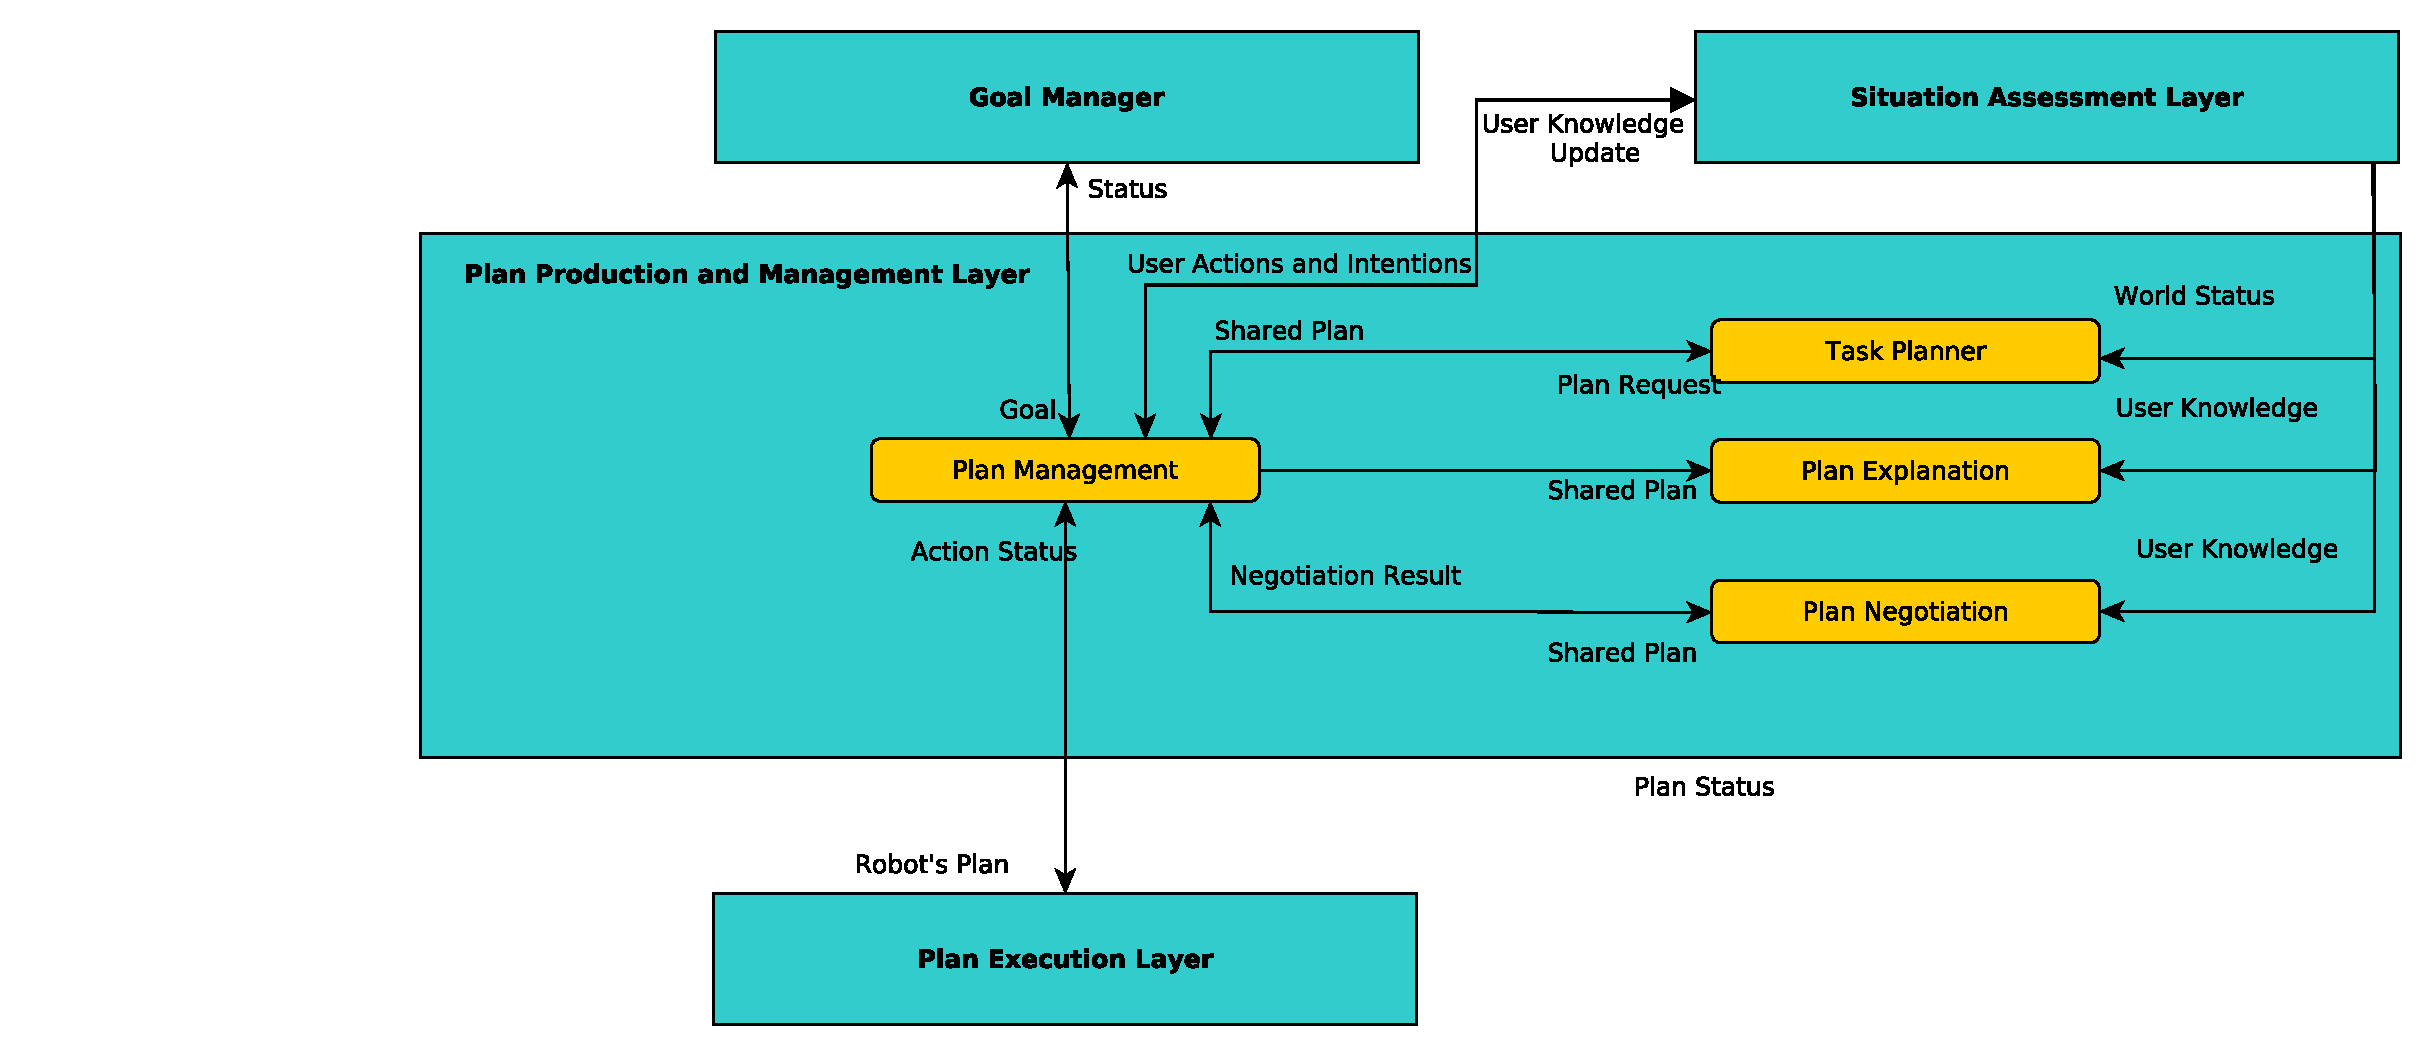
\includegraphics[scale=0.5]{img/plan_management/architecture.pdf}
	\caption[The architecture of the Plan Production and Management layer]{The architecture of the Plan Production and Management layer. Light green rounded rectangles represent modules, while dark green rectangles layers. Arrows represent message exchanged between components, with the label detailing the message.}
	\label{fig:plan_management-architecture}
\end{figure}


Part of this chapter was presented in \cite{Lallement2014,milliez2016using,fioreiser2014}.

\section{Plan Management Modalities}
\label{sec:plan_management-modalities}
When acting together, agents sometimes do not have the same decision power, with one of them assuming the role of a leader. We represent this idea, in our system, by proposing three different modalities: \textit{robot leader}, \textit{human leader}, and \textit{equal qartners}. The robot is able to switch from one modality to another during the execution of a plan. For example, if the current modality is \textit{robot leader} and the Robot receives a command from a user, it will switch to the \textit{human leader} modality, after interrupting its current action.

\subsection{robot leader}
In this modality the robot, after computing the plan, will explain it, negotiate it and start executing it.
The robot will track the status of humans, informing them of which actions they should execute. This modality can be helpful when interacting with  naive users or in tasks where the robot has a better knowledge of the
domain or of the environment than the other agents.

\subsection{Human Leader}
The human can also create plans, interacting with the robot by using a
tablet application, as explained in section \ref{sec:situation_assessment-communication}. In this modality the robot   
will simply observe the surroundings and wait for user inputs. This modality is always available and has a priority over
the other two modalities. If the robot receives a command from the
application while it is in another modality, it will abandon its current
plan, stopping its actions at a safe point, and then execute the users'
command. We feel that this interaction modality is important for two
different reasons.  First, some users will simply prefer to be in
charge of the execution process, for a matter of personal preference or because they
feel they have a deeper knowledge on how to realize the current task
than the robot. We can picture, for example, industrial or medical
scenarios, where the human is the leader and asks the robot to perform
different tasks to help him, when needed. A second use of this modality is in situations where
the robot does not have  a clear estimation of the users' intentions and
goals. For example, in a domestic environment, a user could decide to
order a robot to bring him a drink, a need that the robot can not always anticipate.

\subsection{Equal Partners}
In the last presented operation modality the robot will try to help
the human to complete a task. At the start of the scenario, the robot
will stand still and observe the environment. After the user takes an
action the robot will calculate a plan and try to help as it can, by
performing actions related to that task and by giving helpful information to
the user, for example to fill gaps in their knowledge. In this modality, 
the robot will not explain or negotiate the current plan and will not warn humans if
their actions differ from the plan computed by the robot.

We feel that, particularly in non-critical tasks, where defining an accurate plan between the partners is not
fundamental, this modality is a very natural way of
interaction between different partners.



\section{Human Knowledge and Plan Management}
\label{sec:plan_management-human_knowledge}
\subsection{Representing Human Knowledge in a Task}
Among the topics of this chapter, we will consider different ways to use human knowledge in planning issues. In order to do so, we introduce a new property: the human's knowledge of a task, which will be maintained in the Situation Assessment layer. 

This property is represented as a tuple $(human, task, parameters, value)$, where $human$ is a string identifying the subject of this property, $task$ is the name of the related task, $parameters$ is a list of relevant parameters used to describe knowledge in the task, and $value$ is the level of knowledge in the task. Knowledge values can be assigned from the set $[new, beginner, intermediate, expert]$.  For example, we can represent the fact that Bob knows very well how to fix a wheel to a car with the tuple $(Bob, fix\_wheel, car, expert)$. 

Parameters can be deeply linked to the knowledge of a task. In general, we can divide task parameters in two categories:
\begin{itemize}
\item Class-Link. In some situation, knowledge of a task is not linked to the specific instance of a parameter, but to a whole class. For example, we can imagine that if Bob knows how to paint the living room, he will know how to paint every room in a house. We could represent this property as $(Bob, paint, house\_room, expert)$. We can notice that the parameter, in this case, is $house\_room$, representing the class of rooms belonging to a house, and not $living\_room$.
\item Instance-Link. In other cases, instead, knowledge of a task is deeply linked to specific instances of parameters. For example, knowing how to fix the motor of a specific car, would not necessary translate in knowing how to fix the motor of every car.
\end{itemize}

We can also consider some tasks as \textit{common knowledge}, expecting every human to be able to perform them, like, for example, putting ingredients in a bowl. These tasks will be tagged as \textit{common knowledge} and considered as known by any user, no matter the parameters. 

\subsection{Maintaining Human Knowledge in a Task}
%How human update their knowledge
We define four task-knowledge levels for humans, that will lead to different behaviors from the robot.

\begin{itemize}
\item \textit{New}. This value will be used for tasks which have never been performed by the user. If the user observes the task being executed, with an explanation of it, or if he performs it himself, the value will be changed to \textit{beginner}. However if the user observes the task being executed without any explanation, we keep the level as \textit{new} since we consider that he might not have received enough information to link the observed movements to the task.
\item \textit{Beginner}. This value will be used for users who have already achieved the task but may still need explanations to perform it again. If the user successfully performs the task a second time, without asking for explanations, the value is changed to \textit{intermediate}, otherwise it is changed to \textit{new}.
\item \textit{Intermediate}. This value will be used for users who are able to perform the task without guidance. If a \textit{beginner} user successfully performs the task without guidance again, the value is changed to \textit{expert}. In case of failure, it is downgraded to \textit{beginner}.
\item \textit{Expert}. This knowledge level will be used for users who are able to perform the task without guidance and are experienced enough to explain it to a third party. If the user fails in performing the task, he will be downgraded to \textit{intermediate}.
\end{itemize}

Using the knowledge of a task of a human, the system is able to adapt plan generation, explanation, and monitoring to that user.

\section{Plan Generation}
\label{sec:plan_management-plan_generation}
One of the goals of our system is flexibility; we consider important the possibility to interface with external components. We built an intermediate Plan Generation module that interacts with external planners,  returning  plans represented in a common format that can be handled by the other modules. 

In particular, we require that each planner produces an HTN tree of tasks, showing the decomposition of the plan, which will be helpful in the explanation and monitoring phases; and a set of streams, one per agent, which is useful during the execution of the plan. We introduce casual links between actions, even of different streams, to ensure synchronization. A casual link $l=(a_1,a_2)$ indicates that action $a_1$ should be execute before action $a_2$. This ensures that all the preconditions to execute $a_2$ are fullfilled. Moreover, if $a_1$ and $a_2$ are executed by different agents, and if there is a shared resource connected to the action, the casual link indicates that the resource will be released by the agent only after $a_1$ is completed. An example of these data structures is shown in figure~\ref{fig:plan_management-plan_structure}.

\begin{figure}[ht!]
 \centering
  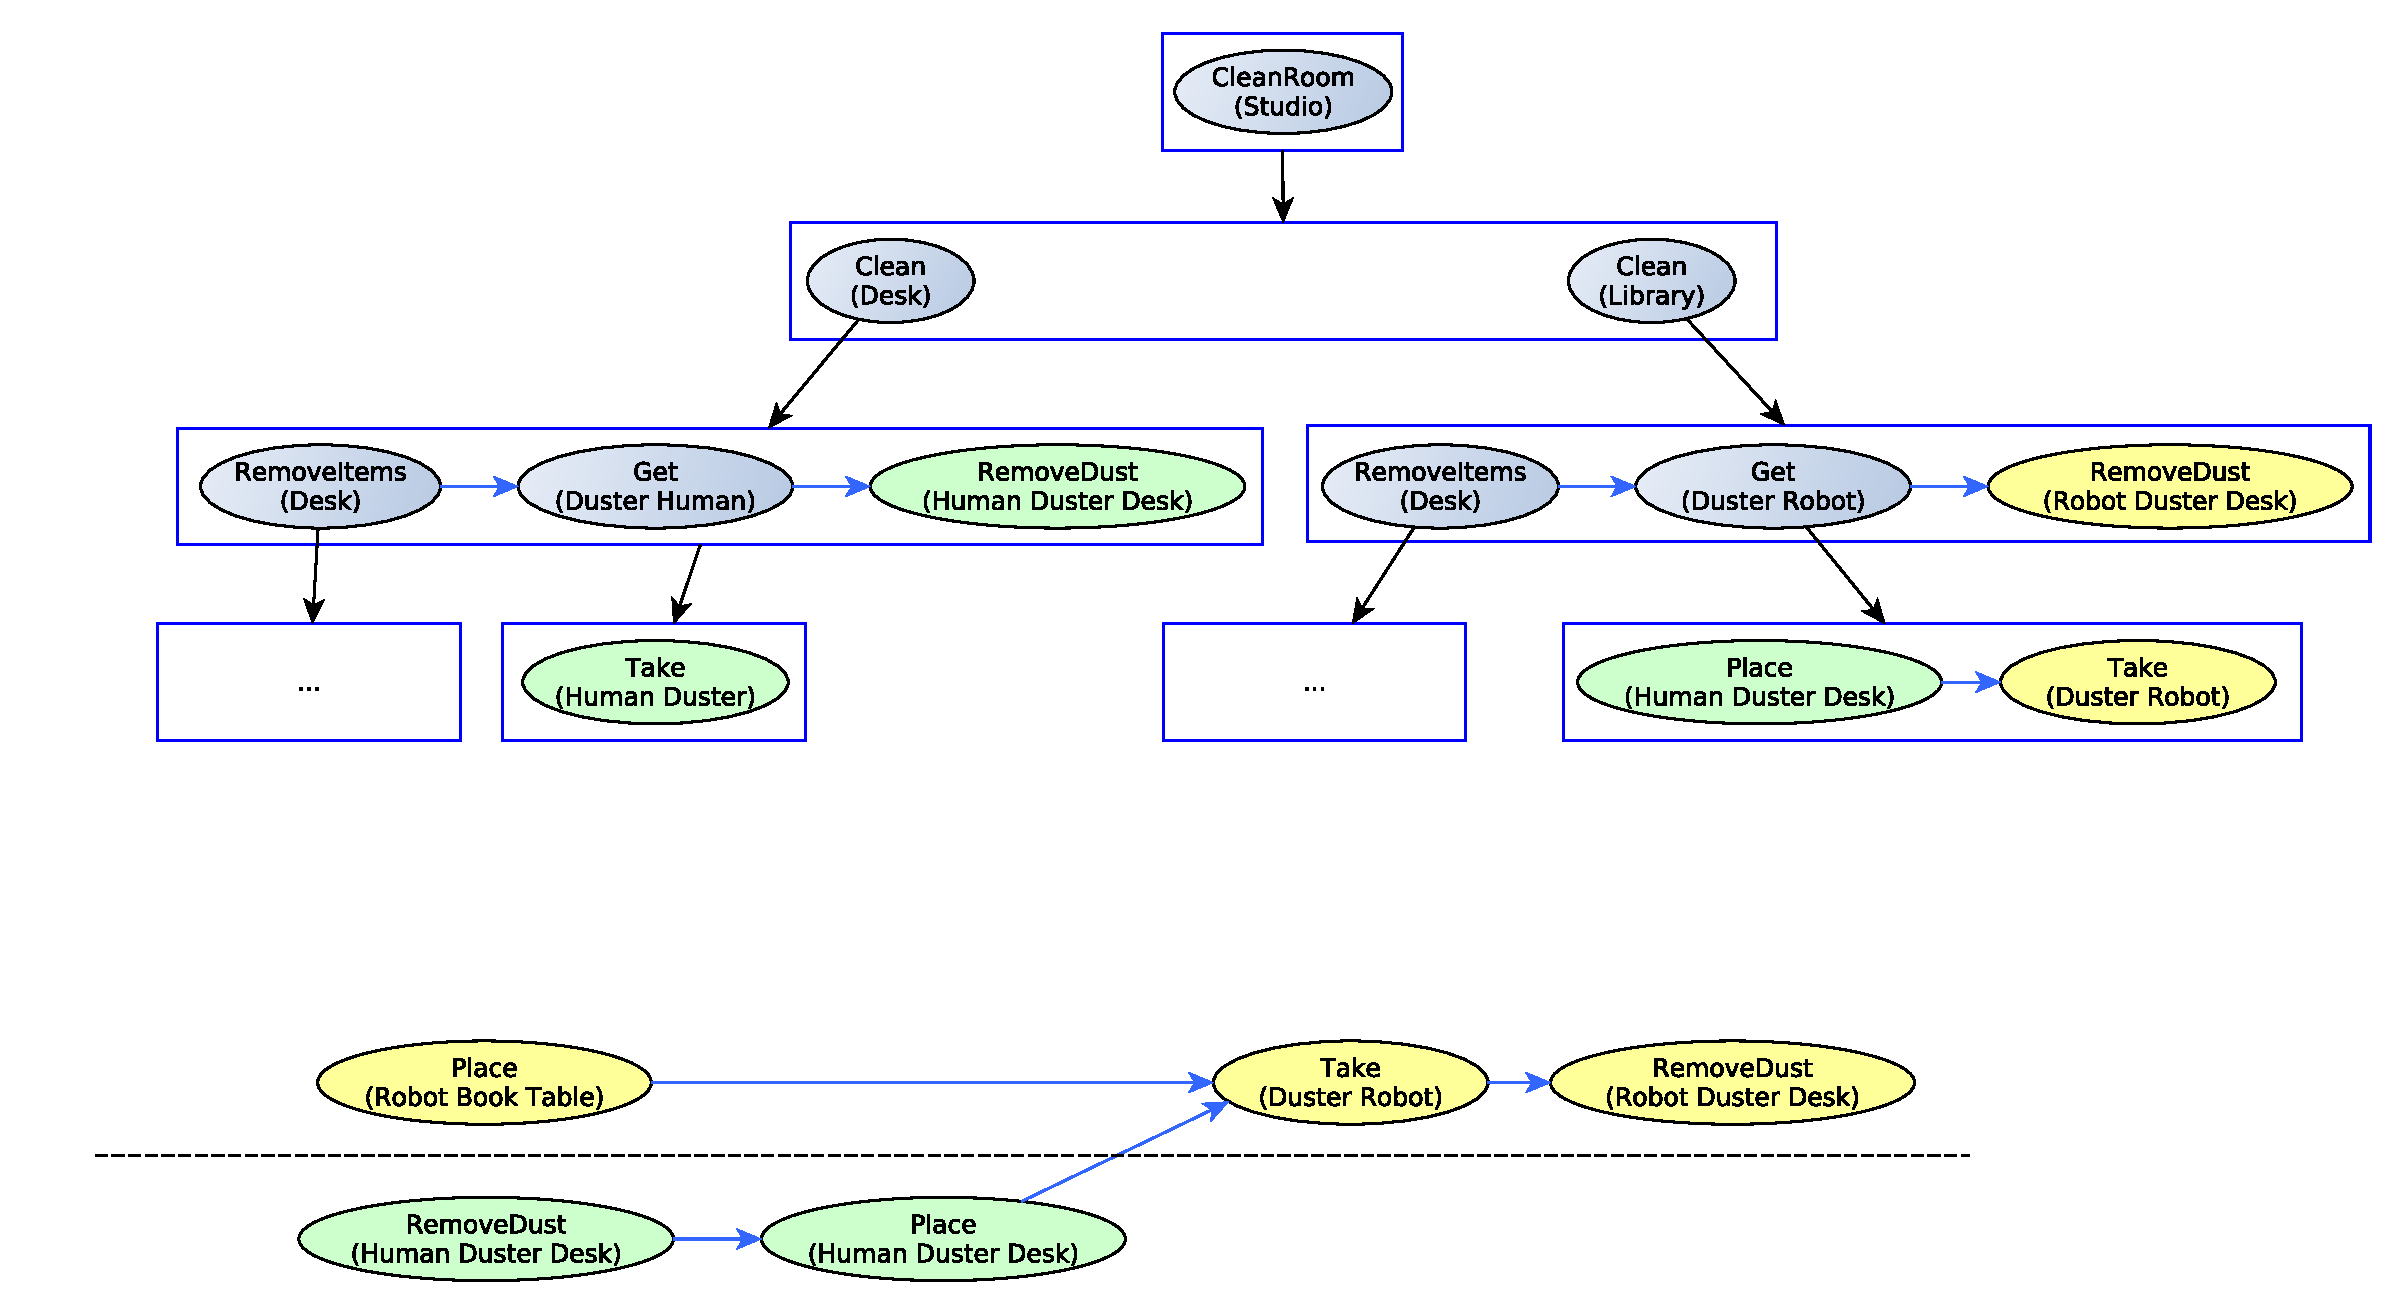
\includegraphics[scale=0.45]{img/plan_management/plan_data_example.pdf}
 \caption[Plan data structures]{a) A HTN plan data structure used in our system, representing a possible way to clean a room
 with two agents, a robot, and a human. Blue ellipses represent tasks, green ellipses represent
 actions assigned to the human, and yellow ellipses actions assigned to the robot. Each decomposition is grouped
 in a blue rectangle. Black arrows link a method to its decomposition, while blue arrows represent casual links. The two squares with a "..." label represent decompositions that are not shown in this picture.
 b) A part of the plan streams associated to the tree data structure. The upper stream represents the robot, and the lower one a human. Notice the casual link between the Place(Human Duster Desk) in the human stream and the Take(Robot Duster) in the robot stream. This link indicates that the robot should wait that the human places the duster before executing the action to take it, ensuring synchronization }
 \label{fig:plan_management-plan_structure}
 \end{figure}


At the moment, we tested two different planners with our system, which will be shown in the next subsections.


\subsection{Human-Aware Task Planner}
\label{subsec:plan_management-hatp}
Computing a plan in complex environments can be very hard and time consuming. A useful approach to reduce the search space in planning is introducing the knowledge of an expert in the system, in order to guide the planner toward desirable states. An implementation of this idea is HTN, where the domain expert specifies a hierarchical library of operations, called methods, when the operation is a node in the hierarchy, and actions, when the operation is a leaf. HATP is a planning framework that extends HTN for human-robot interaction tasks. Among the capacities of HATP we can find:
\begin{itemize}
\item Multi-Agent. HATP is able to plan for different agents at the same time, humans and robots. The planner can also compute ``joint actions", that involves more agents at the same time.
\item Social Rules. The domain expert can introduce a set of rules, which represent desirable behaviors, for example to distribute in different ways operations between agents, or to avoid specific sequences of actions.
\item Cost Driven. The domain expert can specify a cost for actions. Plan pruning allows to explore more efficiently the search space, discarding paths that are not promising.
\end{itemize} 

Plans are represented as an HTN tree decomposition and as a set of streams, one per agent, which shows which actions each agent needs to perform. Casual links are introduced between streams to ensure synchronization.

\subsection{Human-Aware Probabilistic Planner}
\label{subsec:plan_management-happ}

In some situations, agents can work in dynamic environments, and need to constantly adapt their actions to the current state of the world. In this cases, the plan needs to be continuously recreated or repaired, which can be extensive. We deal with this issue we developed a Human-Aware Probabilistic Planner, based on MDPs. Our goal is replicating the characteristics of HATP in a probabilistic domain, so we took the following choices:

\begin{itemize}
\item Centralization. We will use a single planner, which chooses actions for all the involved agents.
\item Hierarchical. The domain will be split in different modules, which interact to solve the issue. Hierarchical models allow us to speed up the computation of the MDP policy, and to reuse models in different domains and tasks.
\item Tightly Coupled. We will focus on problems where the agent's interaction can be frequent.
\item No Communication. We assume that all the agents have a perfect knowledge on the world state, and plan to deal with knowledge issues outside of the planner. Current planners that try to include communication issues often focus on loosely coupled interactions between the agents, in order to simplify the domain and be able to compute a policy for the problem. Since we choose to focus on tightly coupled problems, we can not use this solution, and so prefer to avoid communication issues at this level.
\end{itemize}

The starting point for this planner was the single agent MDP. We enhanced the classical model with the following capabilities:

Parameters. 

We can define parameters in our MDP, and assign to different values. When receiving the world state, the MDP will use information about the assigned parameters to convert this state, which we will call \textit{real_space}, to the MDP space, which we will call \textit{parameter_space}. 

For example, let's imagine a scenario of a room, with different furnitures and object. Let's define the state space of a generic MDP to take an object in this room. We can consider as variables the location of the agent, \textit{agent_isAt}, which can assume value in the set ${f_1, f_2, f_3}$, where $f_i$ represent a furniture in the room. We can define an object variable, \textit{object_isAt}, which can assume the same values as the \textit{agent_isAt} variable. If we define two parameter variables, \textit{agent} and \textit{object}, and link them to the \textit{agent_isAt} and \textit{object_isAt} variables, we can create a generic MDP which can be used to plan for any agent to take an object in this room.

For example, in the real world, we have two agents, \textit{Bob} and \textit{Greg}, and three objects \textit{glue}, \textit{book}, \textit{smartphone}. If we assign the \textit{agent} parameter to \textit{Bob} and the \textit{object} parameter to \textit{book}, when receiving the complete world state, the MDP will assign as \textit{agent_isAt} the location of Bob, and as \textit{object_isAt} the location of the book, discarding unneeded variables.

Parameters allow us to create smaller, generic MDPs, which can be reused easily.


Macro Actions.

We add to the normal set of actions of an MDP \textit{macro actions}, linked to other MDPs, which allow us to create a hierarchy of MDPs. The transition and reward function of a macro action needs to be computed in a different way, since it depends on the sub mdp, and the action can take several time-steps. Several ways have been studied to compute these functions, like the MAXQ algorithm, presented in \cite{dietterich2000hierarchical}. In this work, we compute these functions as shown in \cite{hauskrecht1998hierarchical}. In general, we decided to create a first implementation using simple, well-known algorithms, and plan to study in the future how to optimize them. We call $macro$ the set of macro_actions of the MDP, and $sub(a)$ the sub-MDP linked to action $a$.


Abstract States.

In some situation it can make sense in a model to group a part of the values of a variable. Imagine, for example, the case where an agent needs to perform a series of operations on the furniture $f_1$ in the room. In this case, we could model the  values of the \textit{agent_isAt} variable as ${f_1 , other\_location}$, greatly reducing the state space. In this situation we say that \textit{agent_isAt} is an \textit{abstract variable}. We build a map $abstract_values$ for each abstract variable, which links real world values to values of the model (e.g. $f_2 \rightarrow other\_location$). This map will be used to convert from the $real_space$ to the $parameter_space$ of the model. Teh choice of using abstract variables needs to be carefully weighted, because abstract variables can impact on the quality of the solution of the model.


Now we will explain how we build a Multi-Agent MDP (MAMDP), starting from $n$ single-agent models, one for each agent. 

\begin{itemize}
\item $S=(\bigcup_{i=1}^{n}S_i \ par(S_i))\cup \bigtimes_{i=1}^{n}par(S_i)$, where $S$ is the state space of the MAMDP, $S_i$ is the state space of the agents MDPs, $n$ is the number of agents, $par(S_i)$ is the parameter variables of the $ith$ MDP. We defined the state space of the MAMDP as the union of the state spaces of its single-agent MDPs excluding their parameter variables. For the parameter variables we will do the cross product of those of the single agent MDPs, renaming them to add a string to identify its agent (e.g. \textit{object} will become \textit{objectp1} for the first MDP). We make this choice because parameters could be assigned to different values in the two single agent MDPs, and so need to be treated as separate variables even if they have the same semantic meaning.
\item $A=(\bigtimes_{k=1}^{n} A_k) \cup JointActions$, where $A_k$ is the actions set of the agents MDPs, and $JointActions$ is the set of collaborative actions. The actions of the MAMDP are a concatenation of the actions of the single MDPS. We add to this the special set of $JointActions$, which are actions that the agents can use to cooperate. For example, if there is a resource in a single agent MDP which two agents can possess, we introduce a $handover$ action between the two agents. For each $a_i \in A$, if there is a sub-action $a_{ki}$ of agent $k$ which is a macro action, we create a new MAMDP and assign it as sub-mamdp of $a_i$. This sub-MAMDP will be created from $n$ MDP models, as for its father, in the following way. Let $f$ be the father MAMDP, $s$ the sub-MAMDP, $a$ the macro-action of $f$. $ \foreach MDP m_k \in f$ we assign an MDP $m_j$ in $s$ where:\\
$m_j= \begin{cases}
	m_k & & \quad \text{if } a_{ki} \not\in macro_{k} \\
	sub_k(a_{ki}) & \quad \text{if } a_{ki} \in macro_{k}
\end{cases}$ \\
where $macro_k$ is the set of macros of mdp $m_k$ and $sub_k(a_{ki})$ is the sub-MDP in MDP $k$ linked to action $a_{ki}$.
\item $T(s_i,a,s_j)=
	\begin{cases}
		\prod_{i=1}^{n}(T_k(s_{ki},a_k,s{kj})   & \quad \text{if } !isIncongruent \\
		0   & \quad \text{if } else
	\end{cases}$ \\
	The transition function is computed in several steps. First of all, the state $s_i$ is converted to the single agent states $s_{ki}$, where $k$ is the index of the agent. Then, the we obtain the probability from the transition function $T_k(s_{ki},a_k,s{kj}$. At the last step we check if the transitions of the different agents lead to an incongruent state (i.e. a state where an object is in two different locations). This is done by converting the states $s_{kj}$ in the \textit{real_space} and checking the values of the different variables. We say that a state is incongruent if two non abstract variables have a different value in the two mdps. If one or both the variables are abstract we check if their $abstract_values$ for the current variable value have a value in common. If not, we consider the state incongruent.
\item $C(s_i,a,s_j)= 
	\begin{cases}
		max_{k=1}^{n}(C_k(s_{ki},a_k,s_{kj}))  & \quad \text{if } s_j \not\in G \\
		\sum_{k} Q_k(s_{ki} \forall s_{ki} \in G_k  & \quad \text{if } s_j \in G
		\\
	\end{cases} $	\\
		 where $C_k$ is the cost function of an agent MDP. The cost function of the MAMDP is chosen by taking the maximum cost of the single agent actions that are executed, if the state $s_j$ is not a goal state. If it's a goal state, we take as cost an estimation of the time required by the other agents to complete their tasks, if they do not cooperate. In this way, we encourage the MAMDP to choose plan where the agents cooperate and do not only try to achieve their goal.

\item $SS=\bigcap_{k=1}^n (SS_k)$, where $SS_k$ is the set of starting states of a single agent MDP. The starting states of the MAMDP is set to the intersection of the single agents starting states.

\item $G=\bigcup_{k=1}^n (G_k) $, where $G_k$ is the set of goal states of a single agent MDP. The goal states of the MAMDP is the intersection of the single agent goal states. The idea of this choice is that an MDP terminates when one of the agent has achieved its goal. At this point, if there is a higher level 
\end{itemize}

The result of this fusion is an MDP, that can be solved with well-known algorithms, like value iteration. A model like this could, in general, be very complex but, using macro actions, parameters, and abstract states we can reduce the state space of the model, making it solvable. 

The action space of the joint model is calculated as the cross product of the action spaces of the single model. When 



\subsection{Adapting Plan Generation to Human Knowledge}
\label{subsec:plan_generation-adapting_knowledge}
When interacting with humans, it is important to take into account others' knowledge and capacities when planning. We consider two different policies for our planner: $teaching$, where the planner will look for plans not known to the human, in order to teach him different ways to achieve a task; and \textit{efficiency}, where the robot will try to maximize the number of human tasks known when creating a plan. These ideas were represented as social rules.

To illustrate our planner and the new social rule let us consider an example where a human and a robot have to cook an apple pie. We can consider all the basic actions of this domain (pick, place, cut, etc.) as \textit{common knowledge}, but the human might not know how to perform all the higher level tasks involved. If our policy favors \textit{teaching}, 
the plan should should choose a decomposition with tasks where the human has a low knowledge level. On the other hand, if our policy is \textit{efficiency} the planner should allocate to the human tasks where he is more competent, so that explanations and mistakes are reduced. Using this rule, the robot is able to adapt its plan generation to the knowledge of the user concerning tasks contained in the shared plan. In figure \ref{fig:plan_management-adapting_plan_knowledge} we show an example of plan adaptation for this task with the two policies, using the mental model in table \ref{table:plan_management-apple_pie_human_knowledge}

 
 \begin{table}
\centering
\scriptsize
\renewcommand{\arraystretch}{1.3}
\begin{tabular}{|c|c|}
\hline
Task & Knowledge Level \\ \hline \hline
Cook(ApplePie) & New \\ \hline
PrepareDough(Bowl Mould) & New \\ \hline
PrepareMixture(Bowl Mould) & Intermediate \\ \hline
PrepareFruits(Apple Bowl Mould) & Intermediate \\ \hline
Bake(Mould) & Intermediate \\ 
\hline
\end{tabular}
\caption[Mental model for a human in the Cook Apple
 scenario.]{Mental model for a human in the Cook Apple
 scenario in figure \ref{fig:plan_management-adapting_plan_knowledge} }
 \label{table:plan_management-apple_pie_human_knowledge}    
\end{table}



\begin{figure}[ht!]
 \centering
  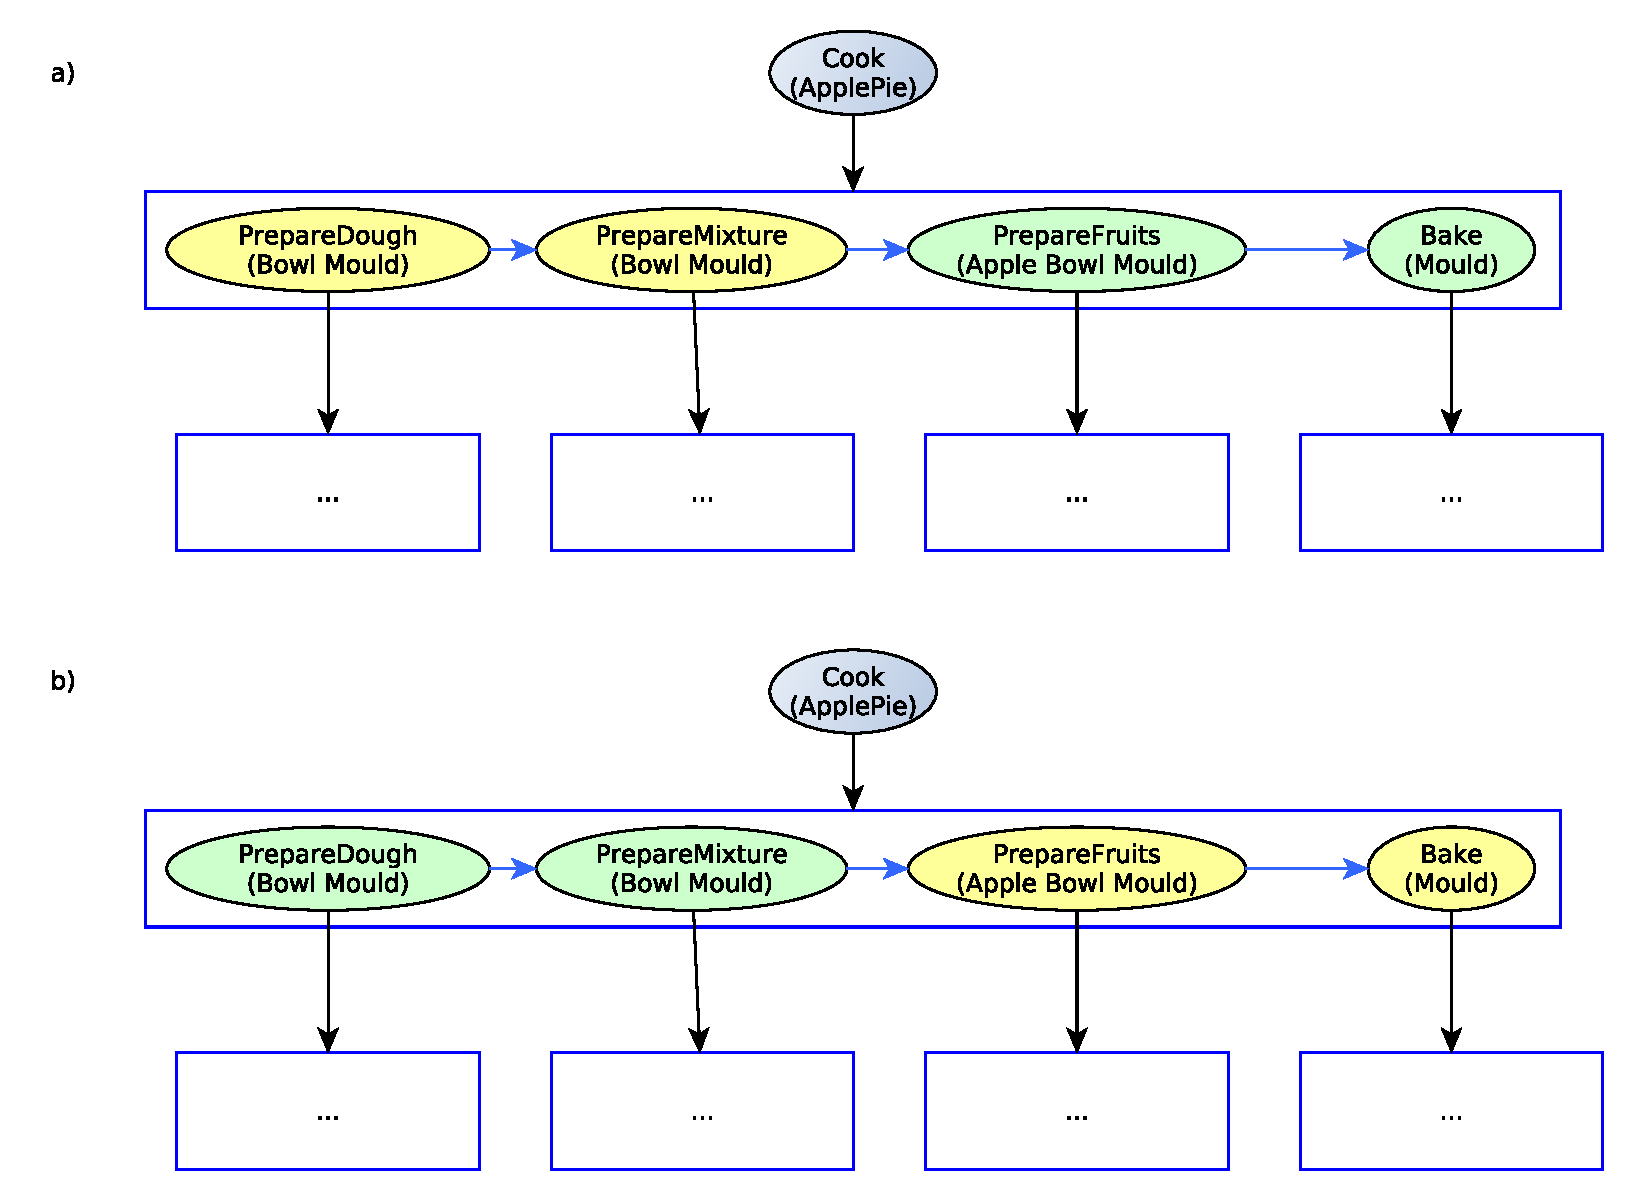
\includegraphics[scale=0.5]{img/plan_management/adapting_plan_knowledge.pdf}
 \caption[Allocation of tasks of a plan to cook an Apple Pie for two agents]{Allocation of tasks of a plan to cook an Apple Pie for two agents, a robot and a human, using the knowledge values in table \ref{table:plan_management-apple_pie_human_knowledge}. A) shows an \textit{efficiency} policy for this task, while b) shows a \textit{teaching} policy for the same task. Blue ellipses represent tasks involving both agents, green ellipses represent tasks assigned to the human, and yellow ellipses tasks assigned to the robot. Each decomposition is grouped in a blue rectangle. Black arrows link a method to its decomposition, while blue arrows represent casual links. Squares with a "..." label represent decompositions that are not shown in this picture.}
 \label{fig:plan_management-adapting_plan_knowledge}
 \end{figure}



To properly compute the cost of a plan, the planner will also upgrade accordingly the knowledge of a task once it is added to the plan. This allows the \textit{efficiency} policy to prefer plans with repetitive decompositions, that are assigned to the same user, over plans with more variable decomposition, where repetitive tasks are assigned to different agents.

The planner can receive information produced from a dialog system that allows to negotiate plans, as explained in section \ref{sec:plan_management-negotiation}. Using this system, the preference and abilities of users are recorded in the Situation Assessment layer. 
If a user is not able to perform a certain task, the planner will never chose this action for him. If he user prefers to perform, or not to perform, a specific task, the planner will update the cost functions accordingly with a reward or penality to assign that task to him.

\section{Plan Explanation}
\label{sec:plan_management-plan_explanation}
Once the system has generated a collaborative plan, if the current modality is \textit{robot leader}, the plan must be shared with the human partners. The robot will present and negotiate plans using speech, which is supported by several studies, such as \cite{Lallee2013,tomasello2005}.

\subsection{Plan Preprocessing}
The HTN generated by the planner represents a solution to achieve the goal. In order to explain this plan to users, the system will process it, removing unnecessary information. In particular, our algorithm follows two rules:
\begin{itemize}
	\item  We remove recursive tasks. If a node $n$ of the tree contains the same method as its parent, $parent(n)$, it will be replaced by its children, $children(n)$. 
	\item We replace nodes with a single child by their children.
\end{itemize}

More formally:
\begin{enumerate}
\item $\textbf{if}$ $(compare(n, parent(n)))$ \textbf{then} $n \leftarrow children(n)$
\item $\textbf{if}$ $(children(n).size() == 1)$ \textbf{then} $n \leftarrow children(n)$
\end{enumerate}

where $compare(n1,n2)$ is true if the two nodes have the same method.

\subsection{Plan Presentation}
Before executing the plan, the robot will present the goal and the proposed allocation of high-level tasks to give a global view of the chosen strategy. Standard natural language generation is used, as shown in table \ref{table:plan_management-pie-present}. 
In some situations, the plan will be too long to explain it at the same time to a user, which could then be confused or annoyed. For this reason, when presenting the plan, the robot will verbalize only the first $N$  highest level tasks. We have chosen $N$=$3$ based on our own experience during tests with the system, but we can imagine to adapt it to the complexity of the domain, or even to specific users. The robot will present the first steps of the plan, perform a negotiation phase, and then execute them. Once these tasks have been executed, the robot will repeat the present/negotiate/execute process until the plan is completed or aborted.
 
 \begin{table}
 %\vspace{-10pt}
\centering
\scriptsize
\renewcommand{\arraystretch}{1.3}
\begin{tabular}{c|c}
   agents(root) $+$ have\_to $+$ root  & "We have to cook an apple pie." \\
   \hline
   introduce\_presentation & "I will tell you the steps." \\
   \hline
   agents(child[0]) $+$ first $+$ child[0] & "You will first fetch the ingredients," \\
   \hline
   then $+$ agents(child[1]) $+$  child[1] & "Then I will assemble the apple pie," \\
   \hline
   finally $+$ agents(child[2]) $+$  child[2] & "Finally, you will bake \\
   & the apple pie in the oven." \\
\end{tabular}
\caption[Presentation of a plan to cook an apple pie]{Presentation of a plan to cook an apple pie. Root is the root of the HTN tree and child is a list with its children.}
 \label{table:plan_management-pie-present}    
\end{table}

\section{Plan Negotiation}
\label{sec:plan_management-negotiation}
Once the robot has presented the plan to his collaborators, it can start a negotiation phase. 

We introduce a simple negotiation algorithm, that starts with the robot asking humans for approval of the plan, inquiring what is wrong in case of disagreement. We handle two different human requests. First, the user can express his preferences, either to perform a task previously assigned to the robot or to not perform a task assigned to him. The other possibility is to inform the robot that the user cannot perform an action. The system will store these information and try to find a new plan, taking them into account, before starting a new explanation and negotiation phase.
 

\section{Plan Management}
\label{sec:plan_management-plan_manager}

Once the plan has been accepted, the agents can start executing it. The three different plan management modalities presented imply different strategies.


\subsection{The robot is not leader}
\label{subsec:plan_management-robot_not_leader_manager}
In the \textit{human leader} and \textit{equal partners}  modalities the robot should not interfere with the actions of its partner. The Plan Management algorithm will be divided in different threads of execution, one for each agent. We will now explain this algorithm, which is shown in figure \ref{fig:plan_management-manage_plan_not_leader}.
\begin{itemize}
  \item Each thread executes the part of the plan of an agent, composed by $n$ different actions.
  \item For each action, for every casual link $(a_i,a_n$), where $a_n$ is the current action, and $a_i$ is another action, the plan manager waits until $a_i$ is completed, or there is an error. This is handled in the \textit{waitCasualLinks} procedure.
  \item When all the casual links have been satisfied, the execute\textbackslash monitor procedure is called, depending if the thread is managing the robot or another agent. The \textit{executeAction} operation interacts with the Execution Management layer to complete the action, while the MonitorAction operation with the Situation Assessment layer.
  \item If these procedures succed, the plan manager switches to the next action, otherwise it returns a failure.
  \item The process is continued until there is a failure or the plan for the current agent is completed.
\end{itemize} 

\begin{figure}[ht!]
 \centering
 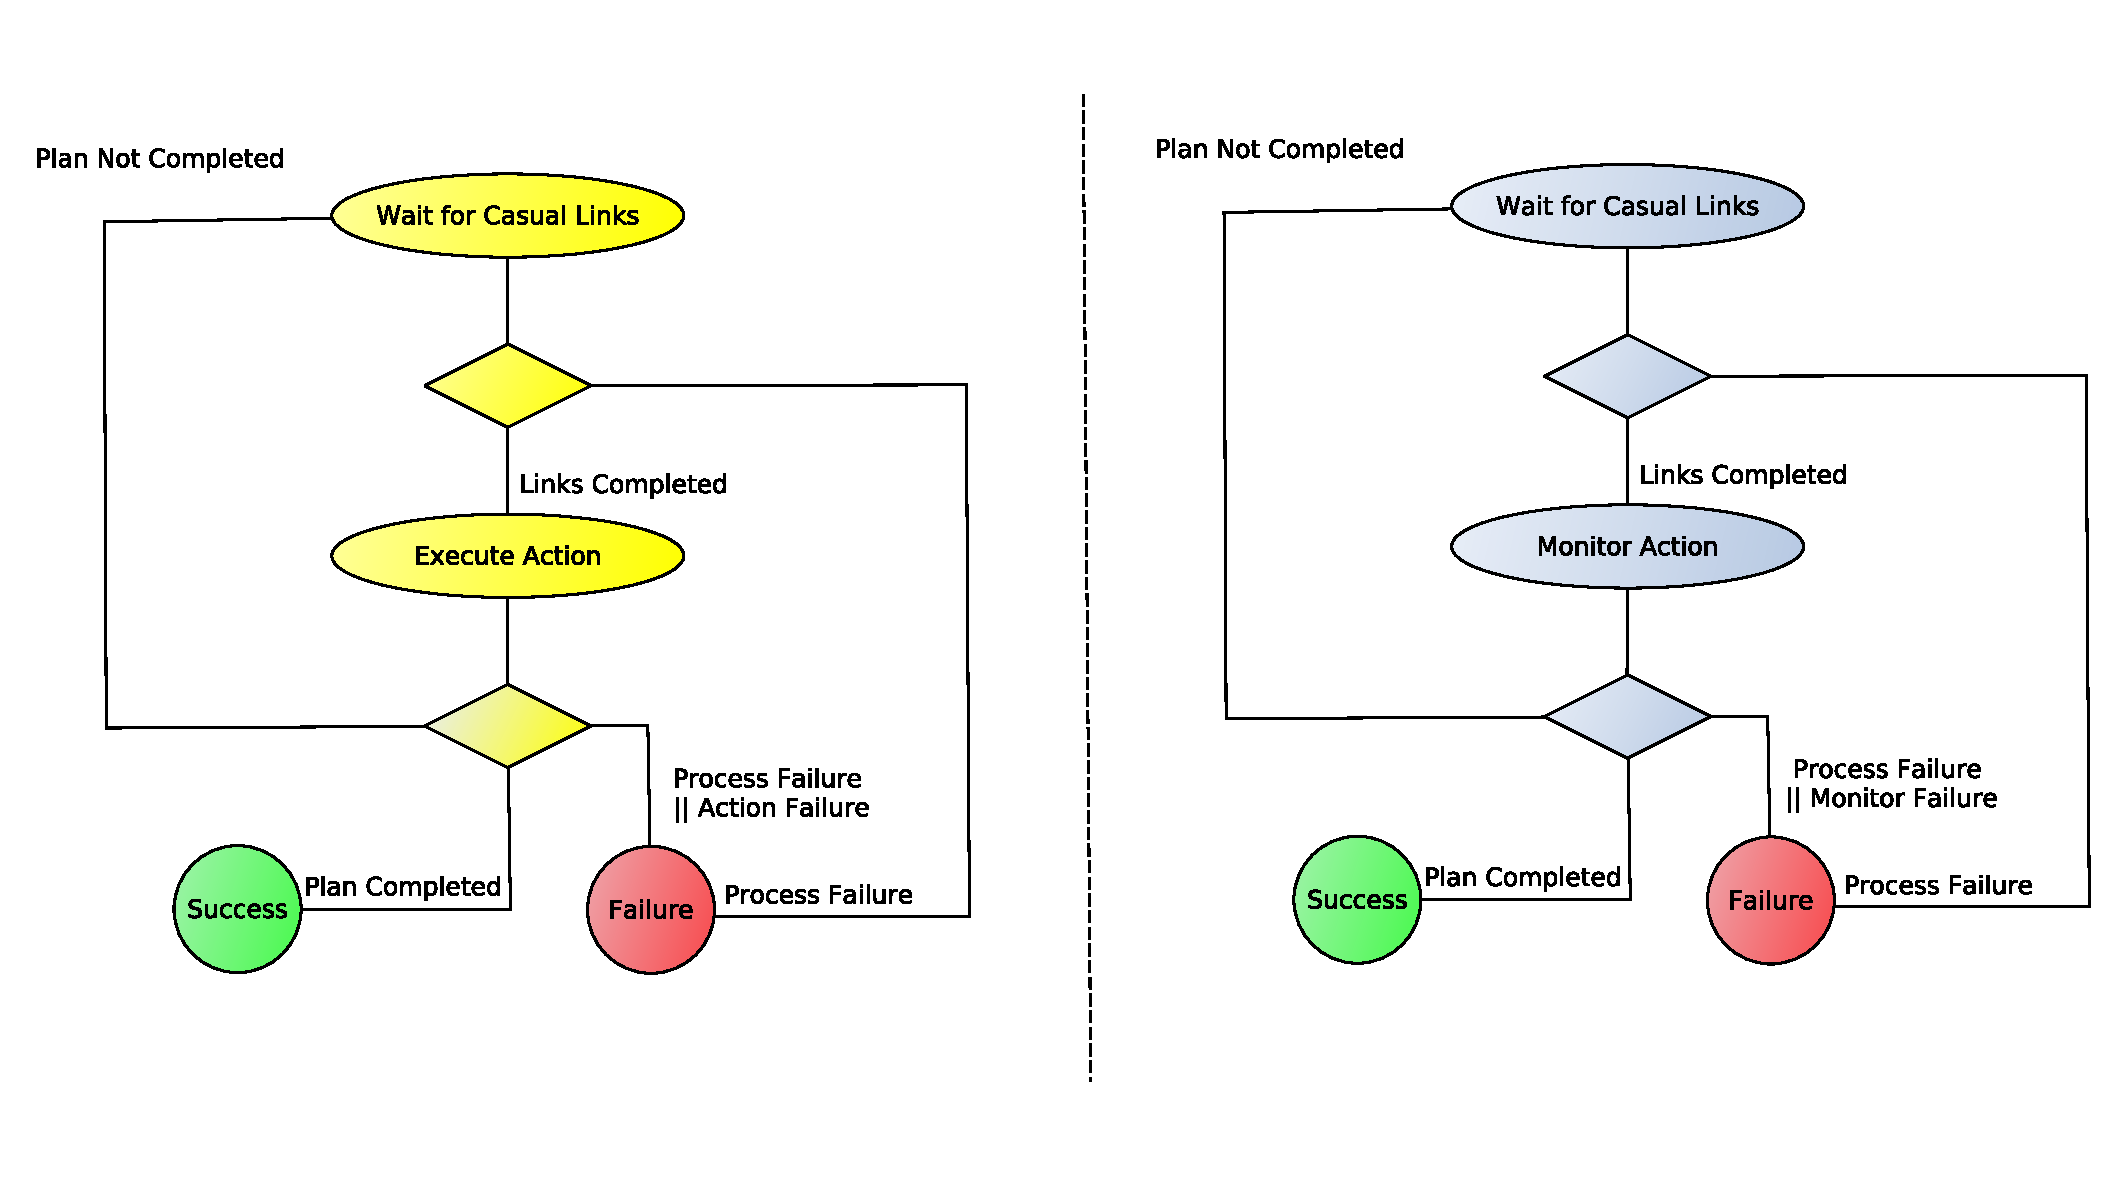
\includegraphics[scale=0.6]{img/plan_management/manage_plan_not_leader.pdf}
 \caption[Plan Management when the robot is not leader]{The plan management algorithm used when the current modality is not \textit{robot leader}. The algorithm is composed by different threads, one for each agent. In this instance, the upper lane represents the robot's management thread, while the bottom a human's management thread. Elliptic nodes represent operations. Diamond nodes, representing divergences in the algorithm, where adding only when they could simplify the understanding of the algorithm. Arrows imply a transition between nodes, with the label of the arrow representing the condition of the transition, when present. The absence of a label implies that a transition is always applied. The blue circle node, called ``start", represents the start of the algorithm. The green and red circle node, instead, represent the success or failure of the algorithm.}
 \label{fig:plan_management-manage_plan_not_leader}
 \end{figure}

Failures in the algorithm lead to a replan request. If a new plan is found, the algorithm starts again, otherwhise the goal is considered failed.

\subsection{The robot is leader}

In the \textit{robot leader} modality the situation is more complex. The plan needs to be analyzed and potentially integrated with ``explanation actions", used to explain a task to a human. In the plan management algorithm previously explained, the robot expects the human to perform a specific stream of operations, and will replan when he deviates from this stream. In this modality, the robot will expect users to execute a specific set of tasks, warning them if they do not respect this allocation. Sometimes, the robot will choose the decomposition of the tasks that should be executed by a user, but, when the partner is competent enough in a high-level task,  we may want to allow him the flexibility to execute it as he sees fit. 

In this situation, we would like to use information about the task allocation, created in the planning\textbackslash presentation\textbackslash negotiation phases, to avoid to replan when a user is executing a task where we allow him flexibility in a different way from the strategy planned by the robot.  Unfortunately, this approach poses several problems. In fact, there might be conditional dependencies between actions of the robot and of the human in the original computed plan. If the human follows another set of actions, the coordination process might break. There are different solutions to this problem:
\begin{itemize}
	\item Executing the plan in a sequential way, disallowing parallelism between the agent. This strategy is less efficient, but it might be useful when the robot wants to teach a task to a user.
	\item Not allowing freedom of execution in tasks whose children have conditional links to robot actions. 
	\item Executing the plan while allowing the user to deviate from it, and repairing it when needed. This approach poses different problems. The first one is understanding when a deviation from the plan imposes the necessity of a repair. The second is that the task planner might generate a plan with a different task allocation, which implies that the robot should restart the explanation process.
\end{itemize}

In \cite{milliez2016using} we presented a first version of an adaptive plan management algorithm, based on executing a plan in a sequential way. We present this algorithm in the following subsection, and then introduce a new parallelized version of it, based on plan reparation.

\subsection{Sequential Adaptive Plan Management Algorithm}
\label{subsec:plan_management-sequential_plan_management}
We start this subsection by showing our sequential plan management algorithm, and then we explain it.

%\begin{algorithm}
\begin{algorithmic}[1]
\For{n$:=$nodes.start to n$:=$nodes.end}
	\If{$agents$(n) = \{robot\}}\label{alg:onlyRobotStart}
    	\If{$children(n) \neq \emptyset$ $\wedge$ $user\_kn(n)$ = new\par
        \hskip\algorithmicindent $\wedge$ $teachPolicy$}
        	\State $execute\_tree(children(n))$
            \State $user\_kn(n) :=$ beginner
        \Else
         	\State $execute(n)$
        \EndIf\label{alg:onlyRobotEnd}
    \ElsIf{$user\_kn(n)$ = new}\label{alg:newStart}
     	\State $explain(n)$
        \If{$children(n)$ $\neq \emptyset$}
          	\State $execute\_tree(children(n))$
            \State $user\_kn(n)$ $:=$ beginner
        \Else
         	\State $monitor(n)$
        \EndIf\label{alg:newEnd}
    \ElsIf{$user\_kn(n)$ = beginner}\label{alg:beginnerStart}
      	\If{$propose\_explain(n)$}
          	\State $user\_kn(n)$ $:=$ new
            \State $(\dots)$ \Comment{Same process as new}
        \Else
          	\State $monitor(n)$
        \EndIf\label{alg:beginnerEnd}
    \ElsIf{$user\_kn(n)$ = intermediate\par
    \hskip\algorithmicindent $\vee$ $user\_kn(n)$ = expert}\label{alg:interStart}
      	\State $monitor(n)$
    \EndIf\label{alg:interEnd}
\EndFor
\end{algorithmic}
%\caption{$execute\_tree(n)$}

%\end{algorithm}

\begin{itemize}
\item \textit{$execute\_tree(n)$} is the main plan management function. The function receives as argument \textit{$nodes$}, a list of nodes initially filled with the root's children.
\item \textit{$teachPolicy$} is a boolean that defines if we are in teaching or efficient mode.
\item \textit{$agents(n)$} returns the agents involved in the node \textit{n}.
\item \textit{$verbalize(n)$} will verbalize the current task, using the node context to present it (e.g. using sequential relations such as first, then or finally according to the node position in the list).
\item \textit{$user\_kn(n)$} returns the knowledge level of the user concerning the task \textit{n}.
\item \textit{$propose\_explain(n)$} will lead the robot to propose an explanation for the current task. If the user accepts the explanation it will return true, and otherwise false.
\item \textit{$explain(n)$} launches a procedure to explain the current task to the user. This procedure could be implemented as a script to launch a video, an explanation speech or even to ask an expert to explain the task.
\item \textit{$monitor(n)$} starts monitoring the proper execution of the current node. If the request returns a success, the function will upgrade the user's knowledge and the \textit{$execute\_tree$} function will continue. In case of failure, the function will downgrade the user's knowledge, exit the \textit{$execute\_tree$} function, and return a failure that will result in a replan request and a new execution if a plan is found.
\item \textit{$execute(n)$} works in a similar way to the monitor but sends a request to execute the node by the robot.
\end{itemize}
 
\subsection{Explanation of the sequential plan management algorithm}
This plan management algorithm is based on the structured plan tree computed by the task planner, and on the tasks' knowledge values in the user models. We explore this tree with a pre-order strategy. The algorithm will analyze each node, with several possible outcomes:

\subsubsection{Only the robot is involved (lines ~\ref{alg:onlyRobotStart}-~\ref{alg:onlyRobotEnd})}
If the robot is the only agent in charge of the current node, the collaborator has a knowledge level equal to \textit{new} for the current task,
and the chosen policy for the interaction is teaching, then the robot will execute the subtasks in ``demonstration mode'', meaning that it will verbalize each child task before performing it.

Once the task have been executed, the robot updates the human's knowledge on the current node to \textit{beginner}. The same process will be applied to the tasks' children.  Using this process, the robot will verbalize each (and only) task that needs to be learned by the collaborator.

If the robot is in charge, but the human collaborator's knowledge on the task is different from \textit{new}, or the current policy is efficiency, the robot will verbalize only the high-level task it performs.

If the human is involved in the current node, the robot's behavior will depend on the human's knowledge level for the task, since the human might need explanations.  Explaining a task could be done in several ways: showing a video, asking an expert to explain the it or simply verbally guiding the user, step by step.
\subsubsection{The collaborator's knowledge level on the task is \textit{new} (lines~\ref{alg:newStart}-~\ref{alg:newEnd})}
If the human has a level $new$ for the current task, we explain it.
When verbally guiding the user, if the current node has only one child, we  go deeper in the tree and apply again the corresponding behavior according to the knowledge level. If the current node is actually an operator (a leaf), the system monitors the current action execution. In case of success, the knowledge level for the task is upgraded to \textit{beginner}.

% if beginner
\subsubsection{The collaborator's knowledge level on the task is \textit{beginner} (lines ~\ref{alg:beginnerStart}-~\ref{alg:beginnerEnd})}
 If the human has a level \textit{beginner} for the current task, we ask if he needs explanations. If so, we downgrade his knowledge level to $new$ on the current task and apply the same process as the previous paragraph. If the user refuses explanations, we simply monitor the execution of the current node. In case of success, the knowledge level for the current task is upgraded to \textit{intermediate}. This knowledge level will also be used as default. This way, when the robot does not know the knowledge level of an agent concerning a task, it will just ask him if he needs an explanation and adapt its behavior accordingly.

% if intermediate
\subsubsection{The collaborator's knowledge level on the task is \textit{intermediate} (lines~\ref{alg:interStart}-~\ref{alg:interEnd})}
 If the human has a level \textit{intermediate} for the current task, we verbalize it without proposing explanations, since he has already  succeeded with the plan at least once without help. Also, we do not go deeper in the tree and directly monitor the current task. If the user  fails, we downgrade his knowledge to \textit{beginner}, otherwise we upgrade it to \textit{expert}.

% if expert
\subsubsection{The collaborator's knowledge level on the task is \textit{expert} (lines~\ref{alg:interStart}-~\ref{alg:interEnd})}
 In case of an \textit{expert} knowledge level on the current task, we  proceed as for the previous knowledge level, downgrading the level to \textit{intermediate} if the user makes a mistake and keeping the \textit{expert} level if he performs the task as expected.


\subsection{Adaptive Parallel Plan Management Algorithm}
\label{subsec:plan_management-adaptive_parallel_plan_manager}
In real cooperative operations, a serialized execution is not enough. The most natural way to interact is, in fact, parallelizing the agents' actions when this is possible. We created a new plan management algorithm to address this issue. We will illustrate its main points.

\subsubsection{Plan Preprocessing}
To start, we pre-process the plan streams produced by the Task Planner. Normally, the plan streams only include low level actions. We need to  modify the humans' plan streams to account for high-level tasks to be monitored. In this new plan, we may substitute groups of nodes with one of their ancestors, when the knowledge level of the human of the ancestor node's task is competent enough, and we want to give him flexibility. This new node will only have casual links in its plan stream, imagining that the human will account on its own to coordinate with other agents. If another agent had a casual link on a removed node, we remove this casual link, but remember this information, as we will account for it in the plan management algorithm.

We will, so, analyze each node $n$:
\begin{itemize}
\item We look in the HTN tree for the oldest ancestor of $n$, that we call $a$, where $kn(a) \geq intermediate$. Note that this node must exist, as $n$ is a leaf (since the plan streams are composed only by leaves of the HTN tree), and we consider leaves as common actions, as explained in section \ref{sec:plan_management-human_knowledge}.

\item If $a$ is different than $n$, let $[n_1..n_m]$ be the list of children of $a$. We substite this list, in the plan stream, with $a$. We set the casual links of $a$ with the predecessor of $n_1$ in the stream and the successor of $n_m$ in the stream (if they exit).
\item For each casual link $l$ starting from any node $m$, where $m$ is a node in a different agent's plan stream, we erase $l$, but record this information in a new flag associated to the node, that we call \textit{had\_casual\_link}.
\end{itemize}


\subsubsection{Algorithm}
After pre-processing the plan streams, the plan manager can start executing the current plan. Each stream will be executed in its own thread. First, we will start explanining the robot's algorithm, which we divide in three blocks: a \textit{control} block, which leads the flow of the program, an \textit{action} block, which controls the execution of actions, and an \textit{explain user} block, which manages eventual explanations to users. We will now details each of these block, starting with the \textit{control} block algorithm, shown in figure \ref{fig:plan_management-manage_plan_leader_control_block}:
\begin{itemize}
\item The plan management algorithm needs to execute $n$ robot actions.
\item If the stream receives an explanation request from the Plan Manager of another agent, the algorithm proceeds in the \textit{explain user} block.
\item If the current plan is not completed, and the algorithm did not receive a failure report from another Plan Manager, the system will wait for the casual links of the current action, using the \textit{waitCasualLink} procedure, which was already explained in subsection \ref{subsec:plan_management-robot_not_leader_manager}.
\item If the system receives an error from another Plan Manager, it will fail, prompting a replan. Otherwise, when the casual links are all satisfied, it will transition to the \textit{action} block.
\item If the plan of the robot is completed, but there are still some users acting, the robot will wait for them to finish their plan, limiting itself to provide explanations, if needed.
\item The Plan Manager terminates successfully when all the agents have completed their plans.
\end{itemize}


\begin{figure}[ht!]
 \centering
 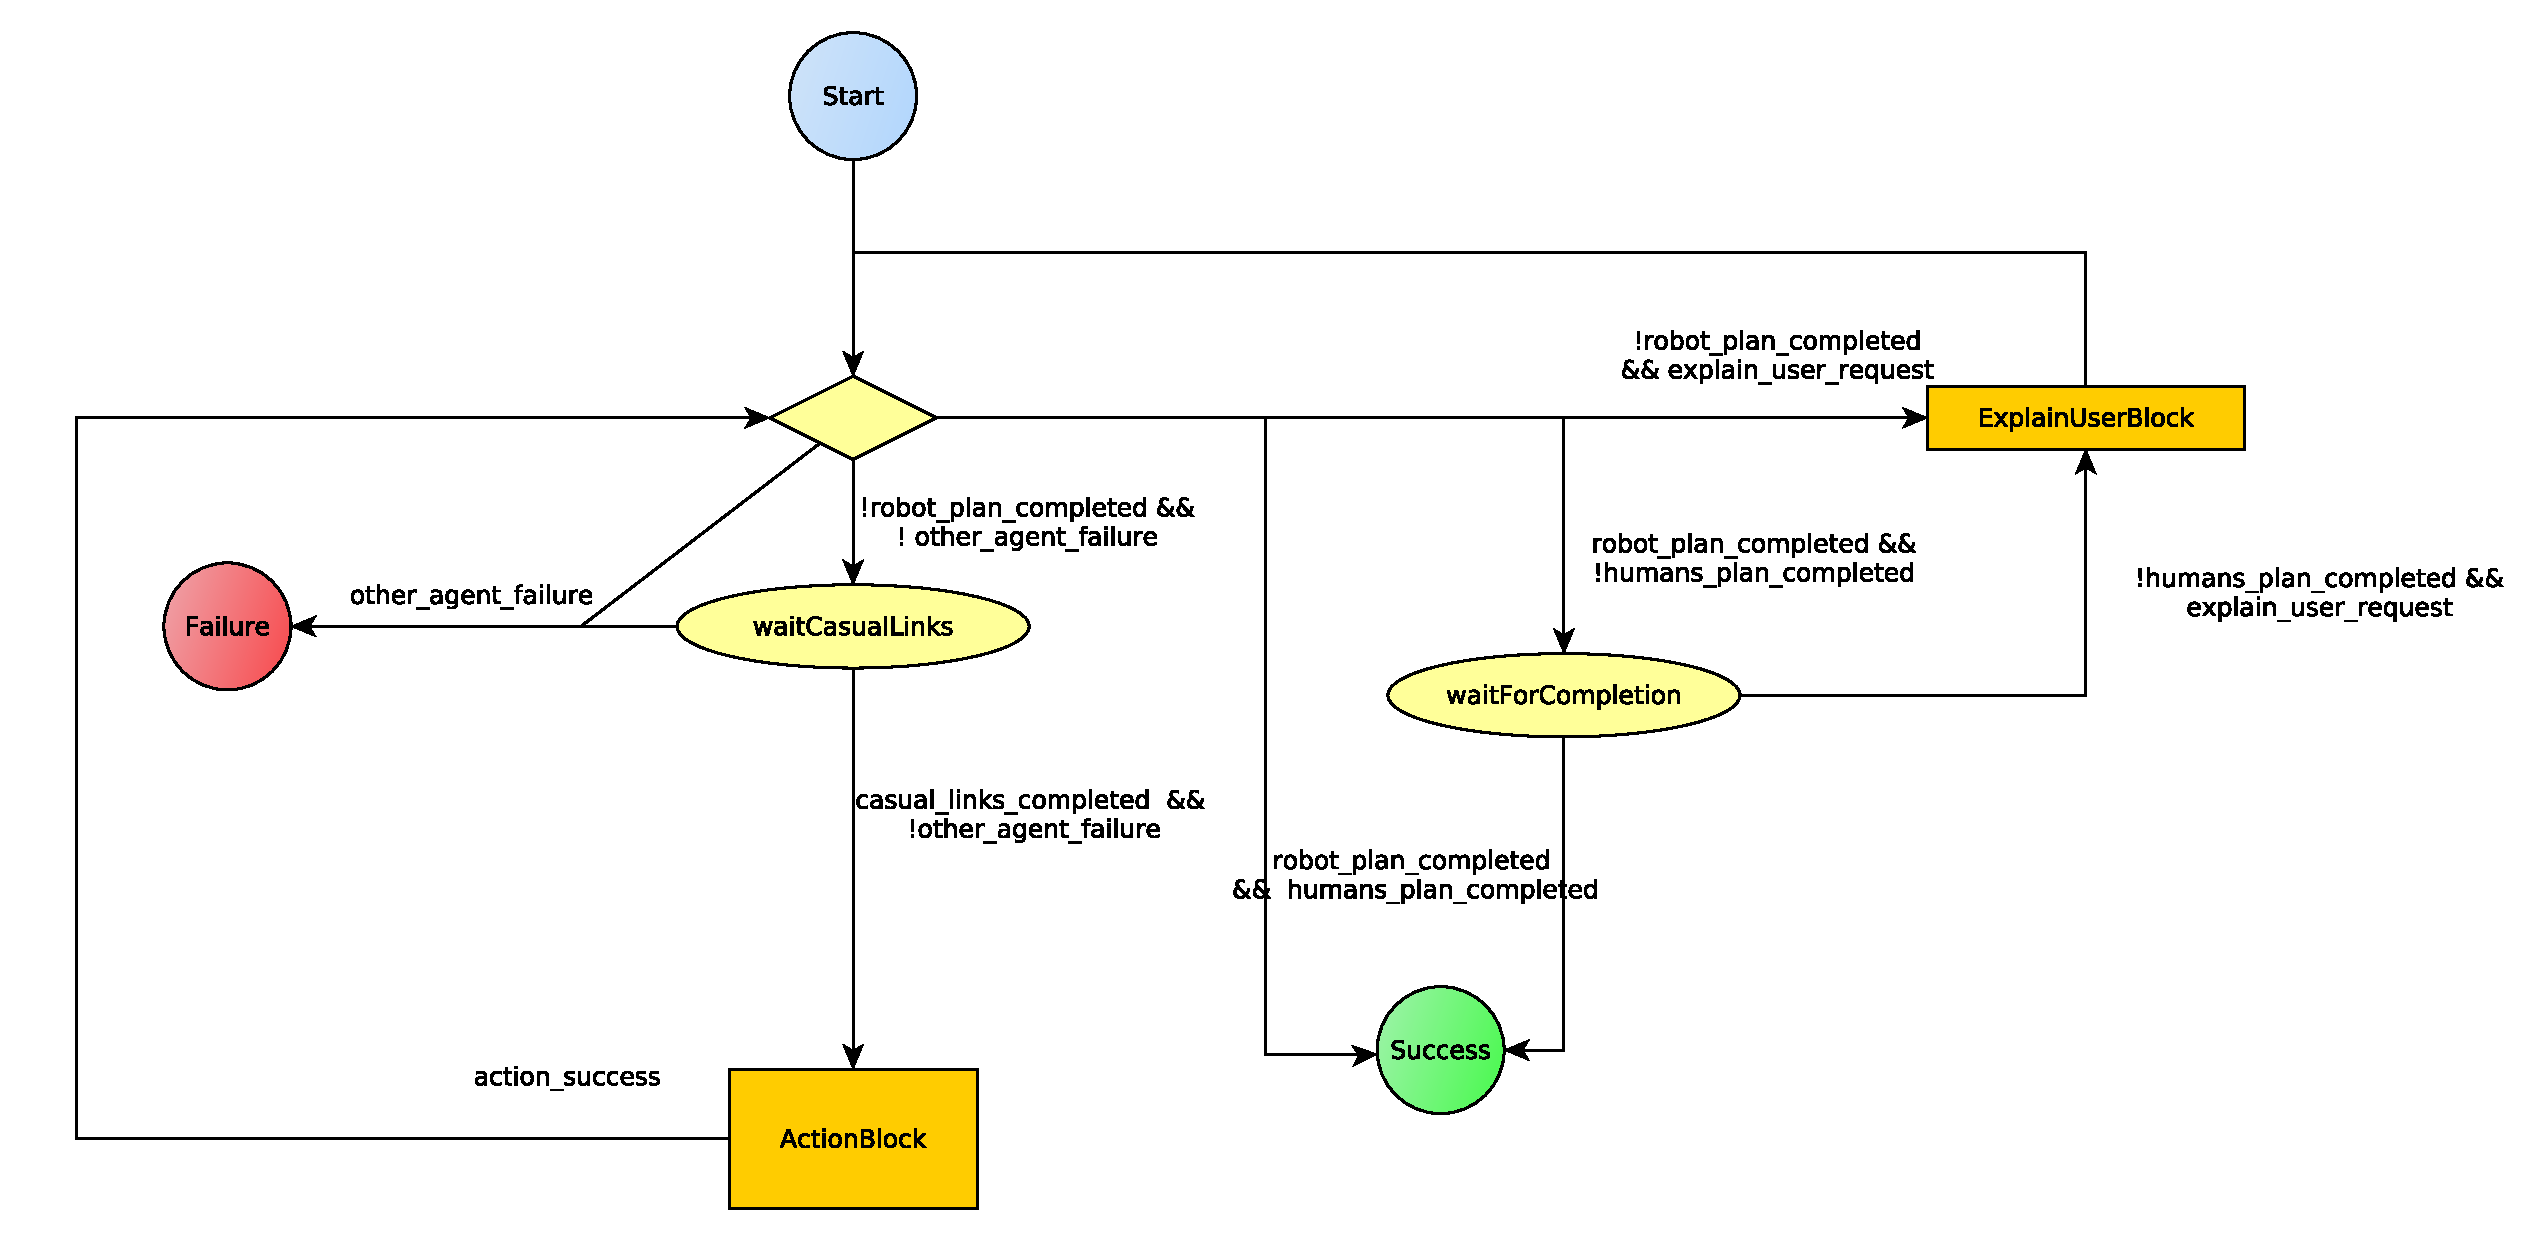
\includegraphics[scale=0.45]{img/plan_management/manage_plan_leader_control_block.pdf}
 \caption[The control block of the parallel plan management algorithm]{The control block of the parallel plan management algorithm used when the current modality is \textit{robot leader}. The symbols used are the same as in figure \ref{fig:plan_management-manage_plan_not_leader}, with the exception of yellow rectangles, which represent other blocks in the algorithm.}
 \label{fig:plan_management-manage_plan_leader_control_block}
 \end{figure}


We continue by explaining the \textit{action} block algorithm, shown in figure \ref{fig:plan_management-manage_plan_leader_action_block}.
\begin{itemize}
\item At the start of this block, the robot will analyze the current action to understand if it needs to verbalize it to users. In order to do so, it will look for the ancestors of the current node in the tree structure, using the same idea shown in the sequential plan management algorithm (lines ~\ref{alg:onlyRobotStart}-~\ref{alg:onlyRobotEnd}). The system will record which tasks have been explained, in order to avoid re-explaining the same task.
\item If the robot should explain some of his actions, it will transition to the \textit{explainAction} function. This function will verbalize the tasks, with the same reasoning shown in the sequential plan manager, if there are users in the same area as the robot.
\item Since the human might take actions that diverge from the robot's plan, the current action might not be executable. Imagine, for example, the case where the robot's current action is to take an object from a table, but that object is not there. There are two possibilities in this case. 1) There was a casual link $(a_h,a_n)$ where $a_h$ is an action that had to be performed by a human, and $a_n$ is the current action. The robot in this case has no way to know if the human has not yet performed the action, or if it will not perform it because he is following a different plan from the one it computed. 2) The human is following a different strategy, making $a_n$ not executable at the moment. For example, the human has taken an object needed by the robot. In this situation, the robot will wait from a predefined time for the action to become executable. If the action does not become executable in this time, the algorithm fails, prompting a replan.
\item If the action is executable but the \textit{had\_casual\_link} flag for $a_n$ is set, the robot will ask the human for permission to perform the action. In fact, we might find situations where the human had to use a shared resource $r$ linked to $a_n$ in the original plan, like an object. The robot can not know if the human is using a different strategy, where he does not need $r$, if he has already finished using it, or if he still needs it. Our solution to this problem is asking him for permission, which is done in the \textit{askPermission} procedure. 
\item If the action is executable, and the \textit{had\_casual\_link} flag is not set, or the robot had permission from the user, the system invokes the \textit{executeAction} procedure, which will go back to the control block in case of success, or return a failure in case of errors. 
\end{itemize}


\begin{figure}[ht!]
 \centering
 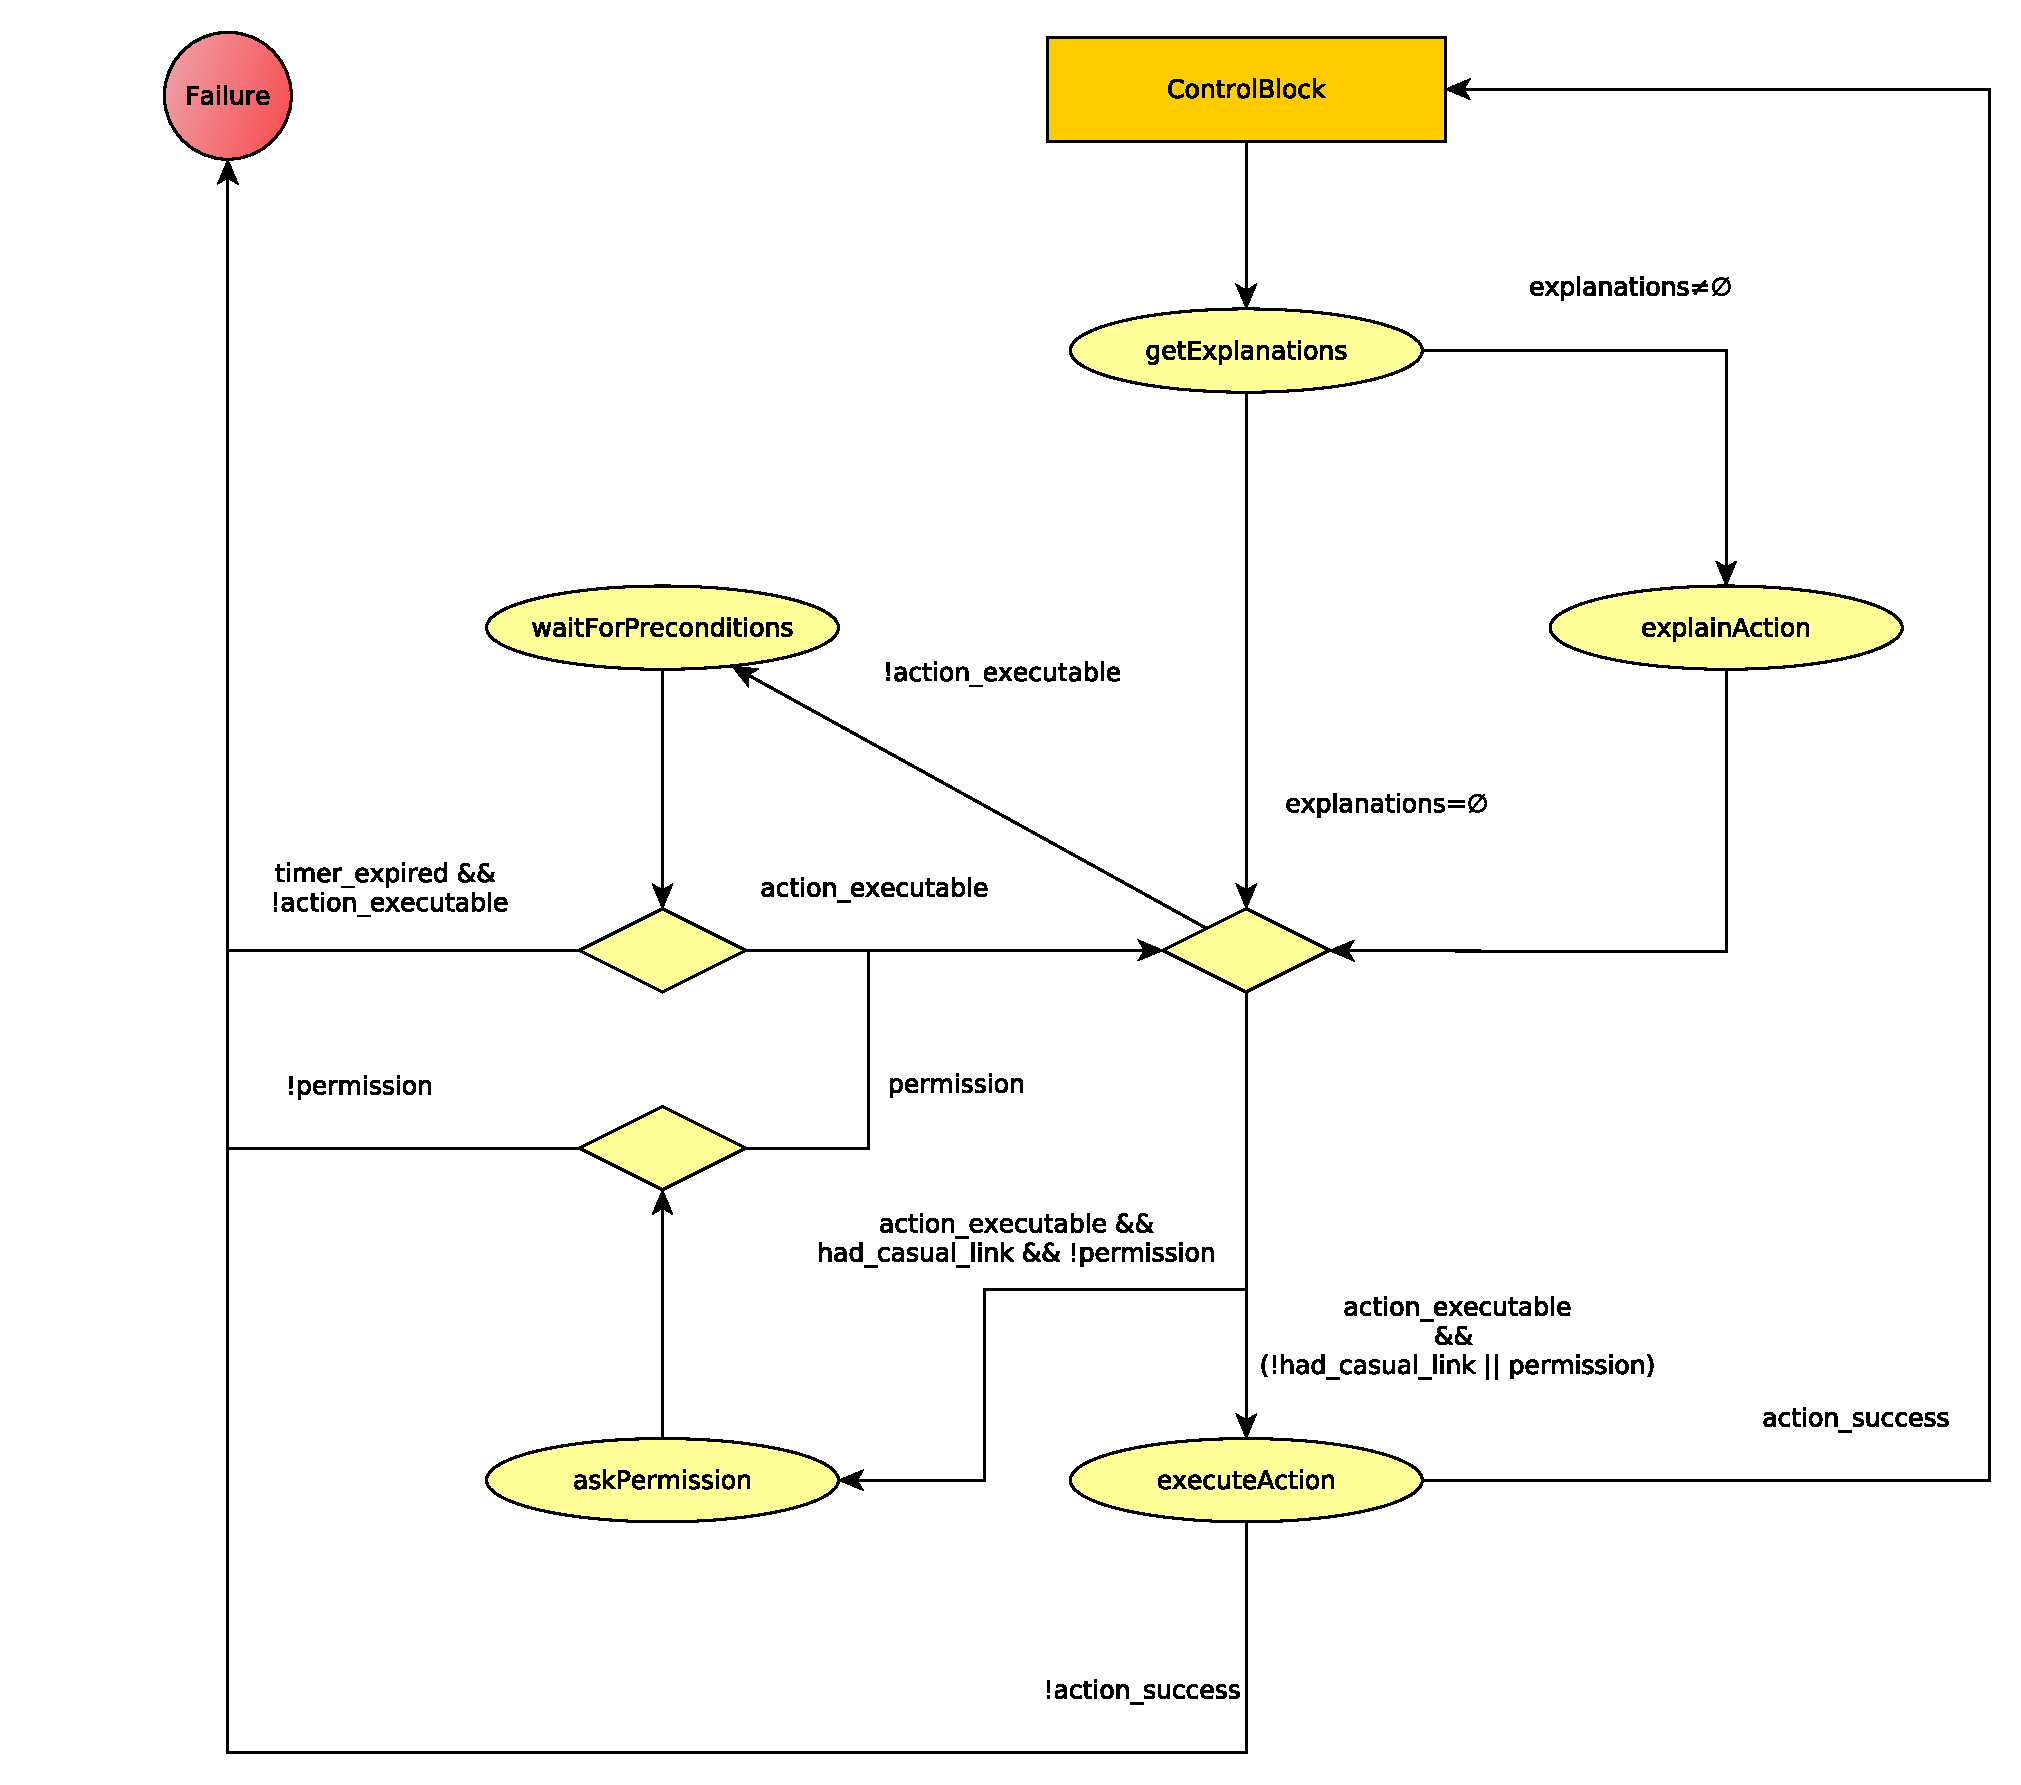
\includegraphics[scale=0.45]{img/plan_management/manage_plan_leader_action_block.pdf}
 \caption[The action block of the parallel plan management algorithm]{The action block of the parallel plan management algorithm used when the current modality is \textit{robot leader}. The symbols used are the same as in figure \ref{fig:plan_management-manage_plan_leader_control_block}. The algorithm starts from the ControlBlock node.}
 \label{fig:plan_management-manage_plan_leader_action_block}
 \end{figure}


Finally, we show the \textit{explain user} block algorithm, shown in figure \ref{fig:plan_management-manage_plan_leader_explain_block}.
\begin{itemize}
\item This block is invoked when the robot's Plan Manager received an explanation request from the Plan Manager of another agent.
\item To start, if the user is in a different location, the robot will move toward him.
\item At this point, if there are no errors, the robot will invoke the $explainUser$ procedure, which might explain him the task, or propose an explanation first, as explained in the sequential plan manager (lines~\ref{alg:newStart}-~\ref{alg:beginnerEnd}). 
\item If the robot changed his position, and his next action in the plan stream is not a $moveTo$ action, which would make it change location, the robot will go back to his previous location.
\item If there is an error during any of these operations, the system will look for a new plan.
\end{itemize}


\begin{figure}[ht!]
 \centering
 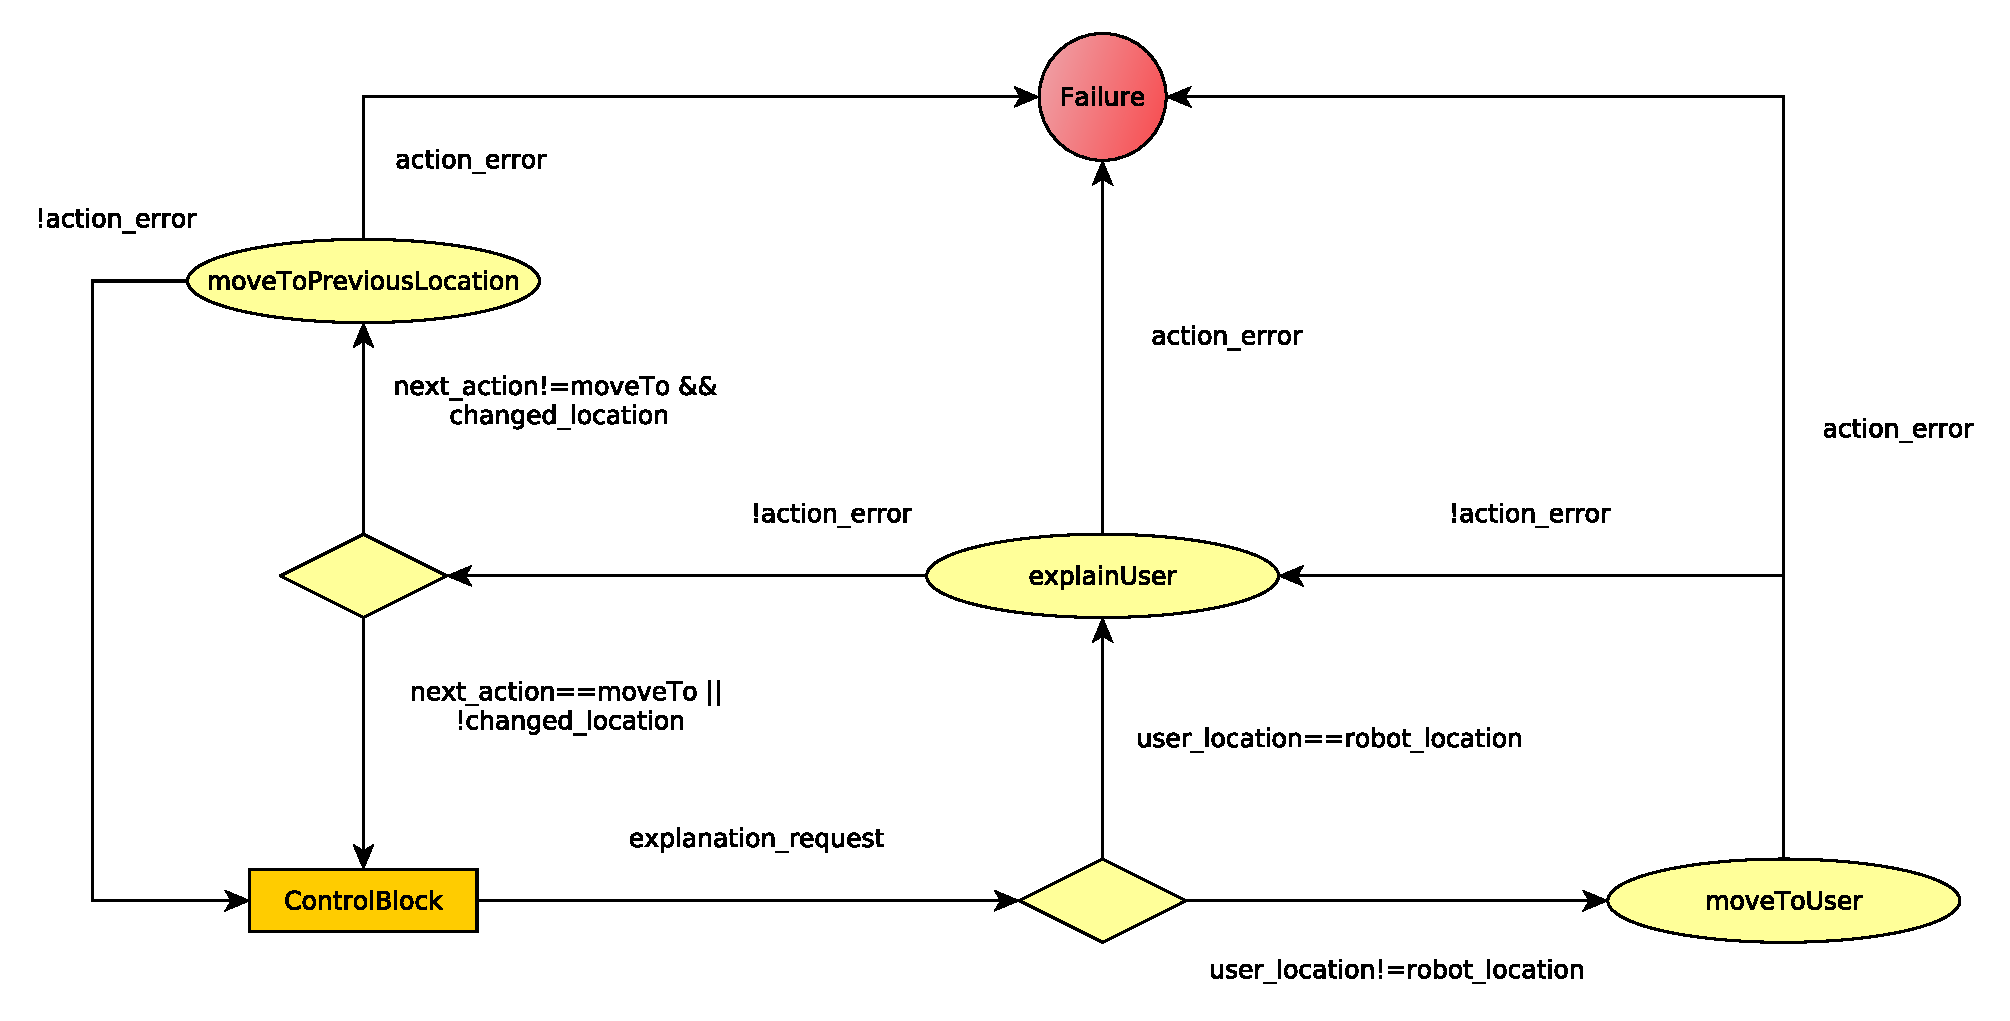
\includegraphics[scale=0.5]{img/plan_management/manage_plan_leader_explanation_block.pdf}
 \caption[The explain block of the parallel plan management algorithm]{The explain block of the parallel plan management algorithm used when the current modality is \textit{robot leader}. The symbols used are the same as in figure \ref{fig:plan_management-manage_plan_leader_control_block}. The algorithm starts from the ControlBlock node.}
 \label{fig:plan_management-manage_plan_leader_explain_block}
 \end{figure}


Now, we will explain the user plan management algorithm, shown in figure \ref{fig:plan_management-manage_plan_leader_humans}
\begin{itemize}
\item This algorithm is, in fact, very similar to the Plan Manager for the other two planning modalities, previously explained in section \ref{subsec:plan_management-robot_not_leader_manager}. The difference lies in the \textit{getExplanations} and \textit{requestExplanations} procedures.
\item The getExplanations procedure is used to decide if the robot should explain the current task of the human, propose an explanation, or simply monitor. This is done analyzing the ancestors of the node, with a similar process to the sequential algorithm (lines~\ref{alg:newStart}-~\ref{alg:beginnerEnd}).
\item If the current task should be explained, the system will send a request to the robot's plan management stream, using the \textit{requestExplanation} procedure. The system will then wait for the end of the robot's explanations or for an error.
\item If there are no errors the system will start monitoring the current task.
\item The process is repeated until the plan is completed or there is an error.
\end{itemize}


\begin{figure}[ht!]
 \centering
 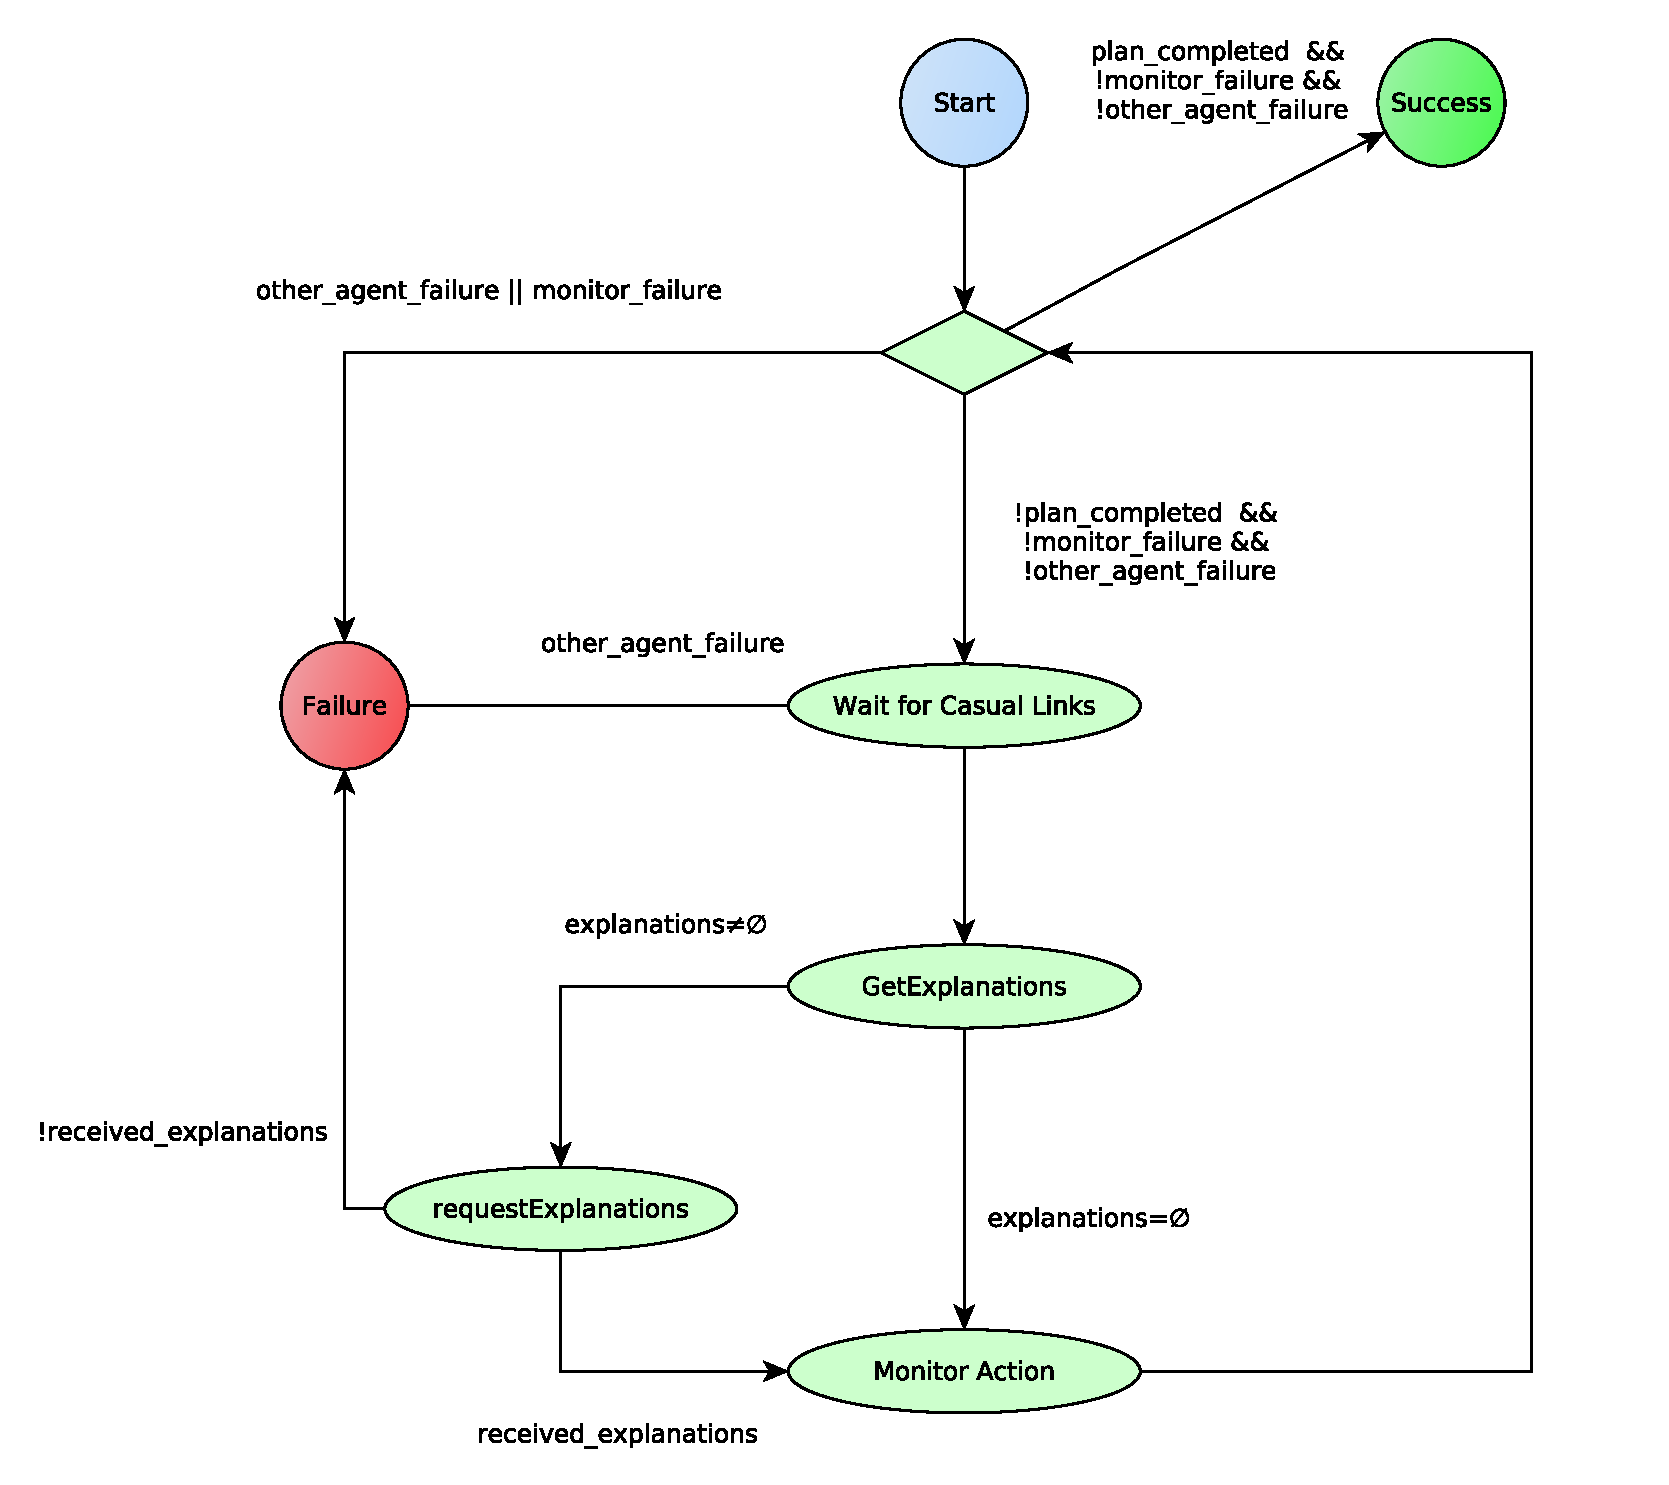
\includegraphics[scale=0.5]{img/plan_management/manage_plan_leader_humans.pdf}
 \caption[The human parallel plan management algorithm]{The human parallel plan management algorithm used when the current modality is \textit{robot leader}. The symbols used are the same as in the previous image, figure \ref{fig:plan_management-manage_plan_leader_control_block}.}
 \label{fig:plan_management-manage_plan_leader_humans}
 \end{figure}


\subsubsection{Human Knowledge and Warnings}
Maintaining human knowledge is done exactly in the same way as the sequential plan manager. The robot will issue a warning to a human when he commits a mistake.

\subsubsection{Replanning}
When the plan manager reports a failure, the system needs to look for a new plan. If possible, we would like to create a plan which contains the same high-level task allocation. Sometimes, when the Plan Manager fails, there is no need to completely change the plan. Instead, it might be sufficient to repair only a part of it. For example, we can imagine a scenario where a human might execute task $t_1$ using resource $r_1$ or $r_2$. Perhaps the robot computed a plan where the human will use resource $r_1$, while itself will use $r_2$ to achieve another task.

If the human does not follow this plan, and uses $r_2$ to compute its task,  it might be faster to just repair the plan, looking for a solution where the task allocation is the same, but the robot uses $r_1$ instead to achieve its task. This way, we avoid starting a new explanation\textbackslash negotiation phase, which could look useless and not natural to the human collaborator.

%  We deal with this issue in different ways in HATP and HAPP.

In HATP, we introduce a new cost rule. When presenting a plan, we record which nodes have been presented and assigned to each agent. While planning, we penalize plans with a different task allocation. This way, the planner will prefer to use the same task allocation, but will change it if needed, for example because, using the previous task allocation, the goal is no longer achievable.

%In HAPP, we can just perform a partial replan, by interrogating the currently active MMODP.  


\section{Plan Monitoring}
\label{section:plan_management-plan_monitoring}

\subsection{Introduction}
During the execution of a plan, the robot will monitor other agents. In general, having a shared plan, the robot knows what is the user's next expected action, and can monitor if it is accomplished. Plan monitoring poses a number of different issues:
\begin{itemize}
\item Understanding when the next expected action has been performed. In some situations the robot will monitor the execution of a specific action. In this event, it needs to understand when the action has been completed.
\item Understanding when the next expected task has been performed. In some situations, the robot wants to give a human cooperator the freedom to perform a subtask has he sees fit. This is a more complex problem than monitoring a specific action, since the robot needs to reason on the results of sequences of actions.
\item Evaluating the human engagement in the current task. The robot needs to understand if the human is trying to accomplish its current task, if he momentarily interrupted it, or if he abandoned it.
\end{itemize}

\subsection{Monitoring Plans}
When executing a shared goal, the Plan Production and Management layer needs to interact with the Intention and Action Recognition module in the Situation Assessment layer. Normally, this module is not able to monitor joint goals, since the inference mechanism presented in subsection \ref{sec:situation_assessment-action_evaluation} is based on single-agent MDPs. To solve this issue, while performing a shared plan, we create, in the Situation Assessment layer, a new intention for each node in the HTN tree whose task can be currently performed (meaning, if it has casual links to other tasks, they have already been satisfied). We associate to these intentions the linked MAMDP, as previously explained in \ref{subsec:plan_management-happ},
 and the context node \textit{have a shared plan}, which is treated as evidence with a true value. We call these intentions \textit{plan intentions}.

We associate to each known intention a precomputed \textit{expected length}, which is the expected time to accomplish the linked goal.

The robot can be updated at each time on what actions have been performed, using the mechanisms described in section \ref{sec:situation_assessment-intention_recognition}. This way, the robot can compare actions that are actually performed by humans with those that \textit{should} be performed following the shared plan.

Using the Intention and Action Recognition module, the robot can infer which is currently the most likely human intention. If the current intention equals the task to monitor, the robot infers that the human is actively working to complete its task. We consider the task, and the monitor procedure, as completed when the linked MAMDP reaches a goal state.

If the human is currently not involved in the monitored task there are three possibilities:
\begin{itemize}
	\item The human has momentarily interrupted the task. This can be inferred if the human is currently involved in another intention, which does not belong to the \textit{plan intentions}, and whose expected length is \textit{short}. In this case, the monitor procedure will not return an error until a predefined \textit{allowed time}.
	\item The human has abandoned the task.  This can be inferred if the human is currently involved in another intention, which does not belong to the \textit{plan intentions}, and whose expected length is \textit{long}. The monitor will return a \textit{not involved error}. 
	\item The human is performing another task in the shared goal. This can be inferred if the human is currently involved in another intention, which belongs to the \textit{plan intentions}. In this case the monitor will return an \textit{other task error}. 
\end{itemize}


\subsection{Monitoring and Unseen Actions}
Often, in cooperative tasks, agents will operate in different locations, and so they can not observe each other actions all the time. Perhaps one of the agents is cooking in the kitchen,  while the robot is preparing the table for dinner. While we do not deal, in this work, with these issues, there are several studies on plan recognition in partially observable environments, like \cite{geib2005partial}.

\section{Experiments and Discussion}
\label{sec:plan_management-experiments}
In this section, we present a set of experiments which where performed to evaluate the performance of the Plan Explanation and Sequential Adaptive Plan Management systems.

 \subsection{Experiment}
 \label{sec:plan_management-experiment}
To test our system, we have chosen a scenario where a human is trying to prepare two desserts, an apple pie and a banana pie, without knowing their recipes. The robot's goal is guiding and assisting the user, as shown in figure \ref{fig:plan_management-scenario}. 

\begin{figure}[ht!]

 \centering
 \begin{tabular}{cc}
  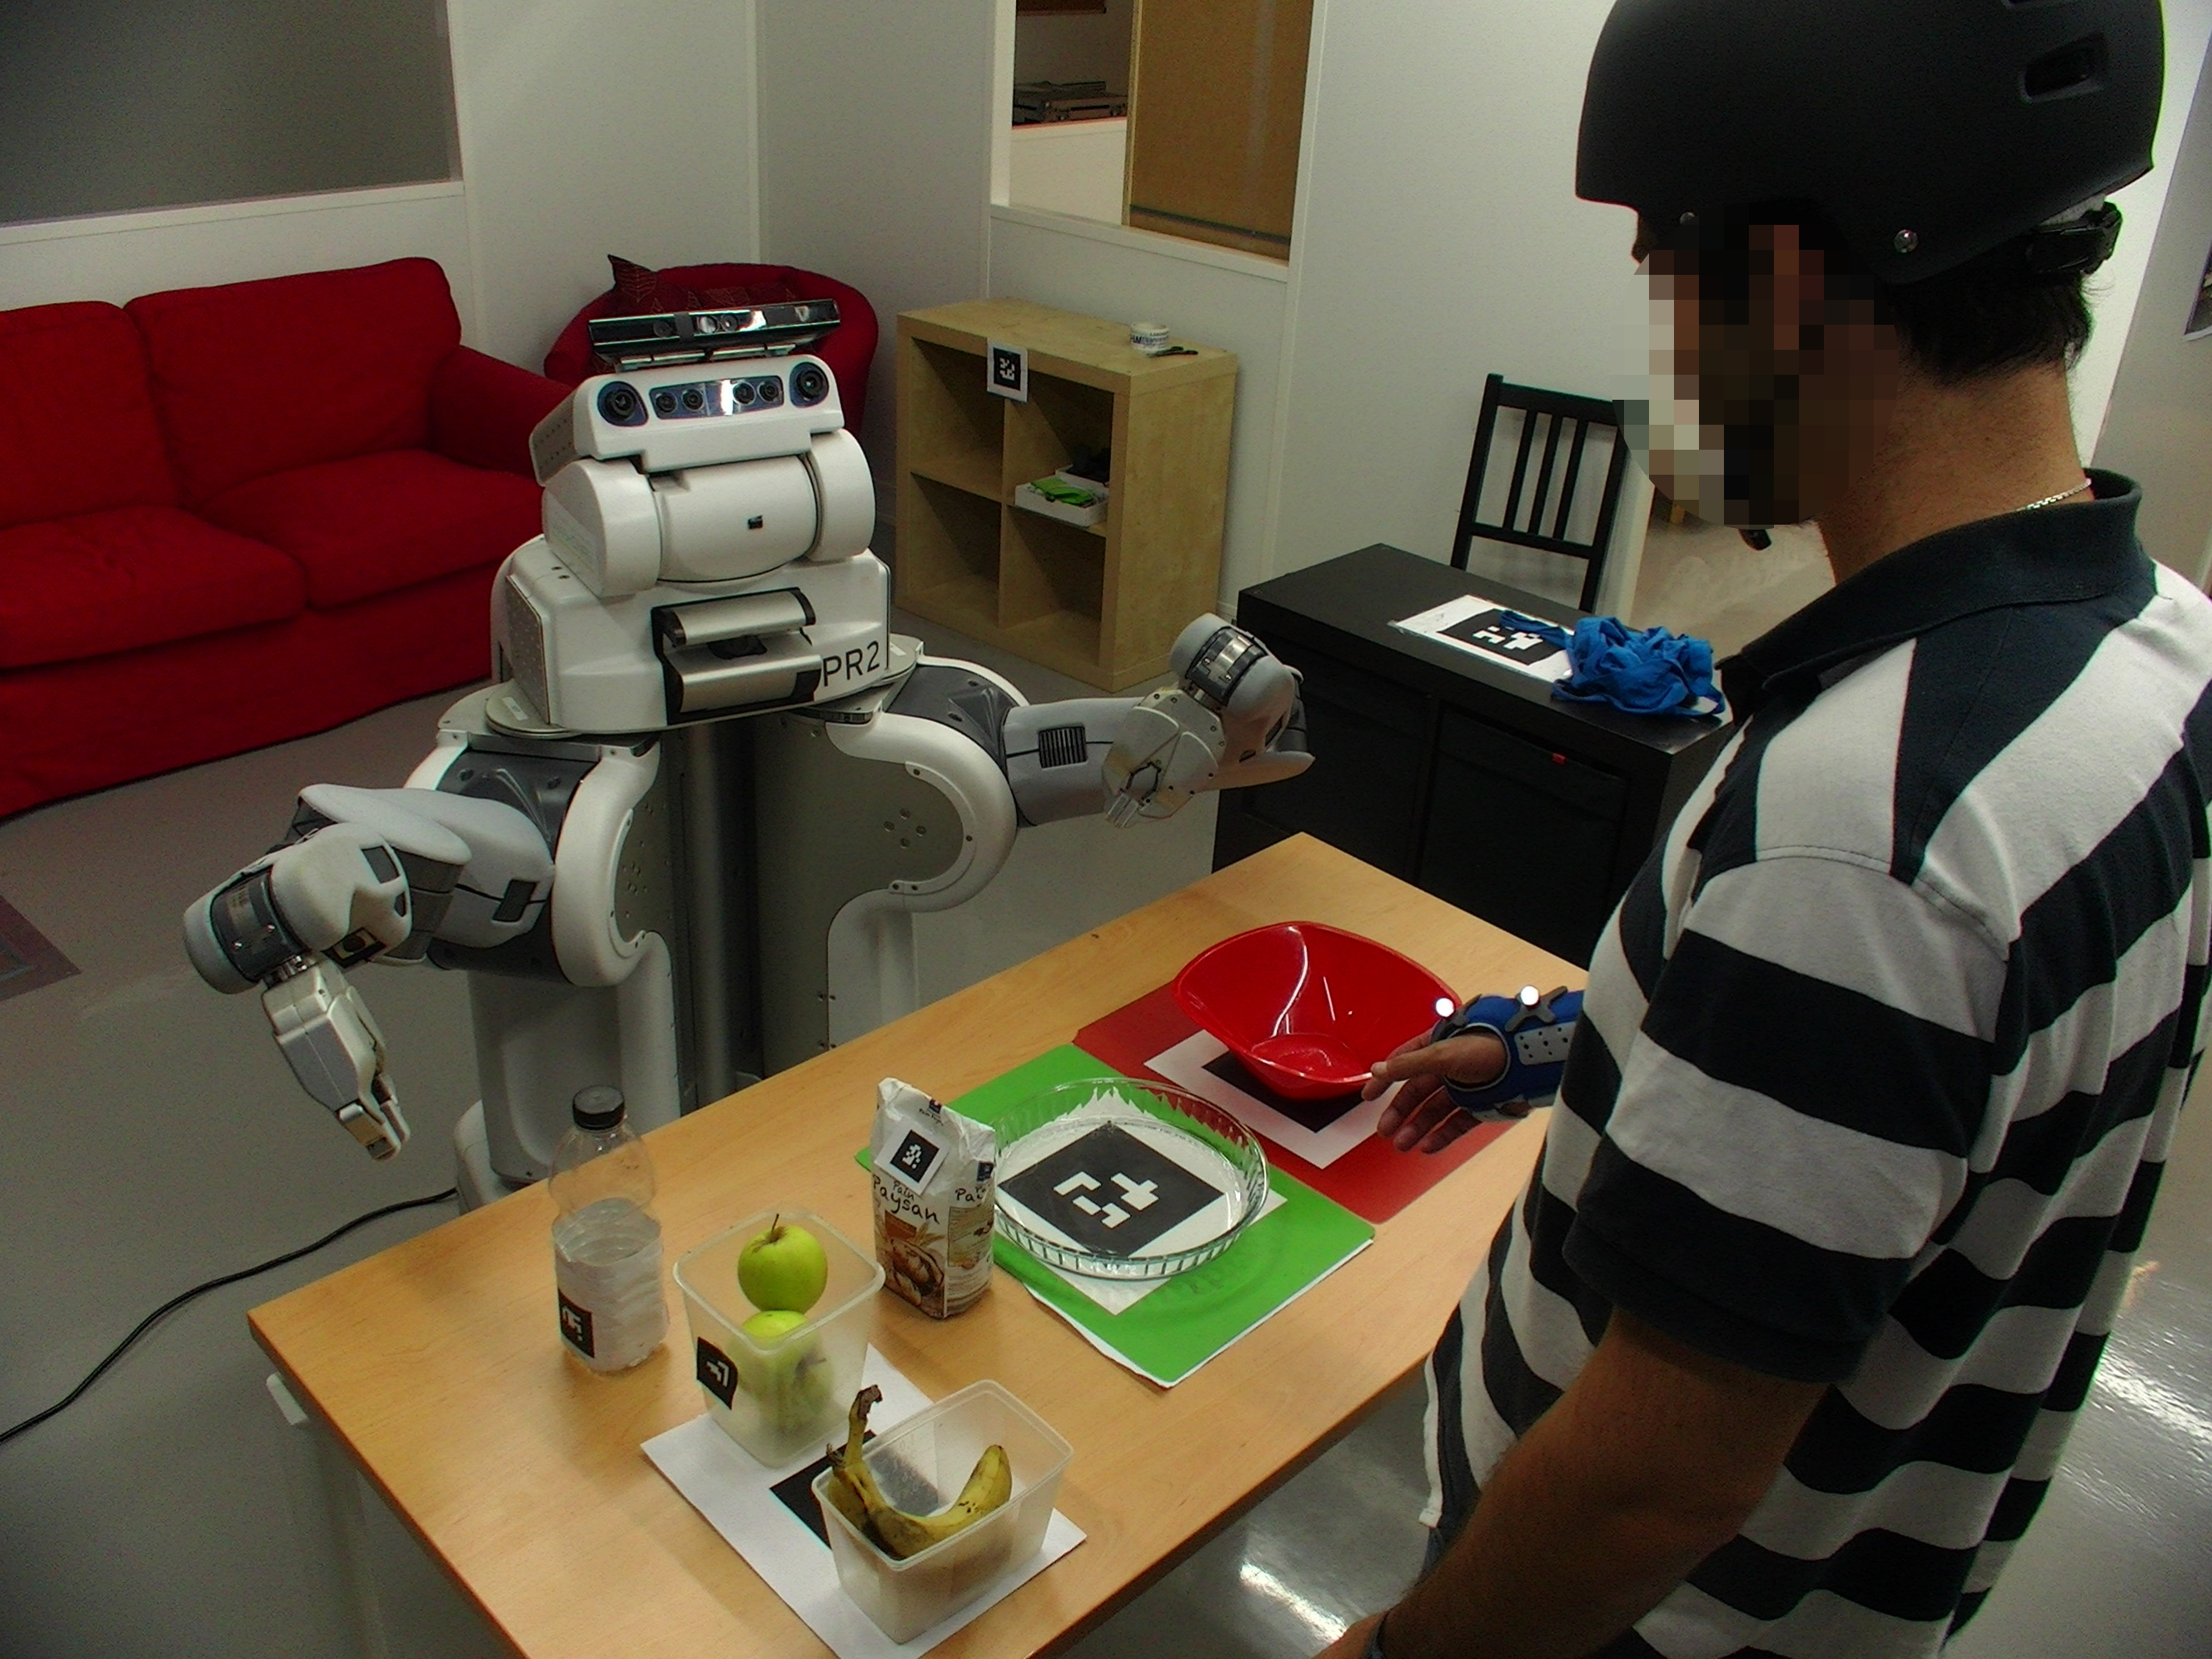
\includegraphics[width=0.29\textwidth]{img/plan_management/scenario.JPG}
 \end{tabular}
 \caption{Illustration of the cooking pies scenario}
 \label{fig:plan_management-scenario}
 \end{figure}

We created a domaint to represent this scenario, and tested it using the previously explained \textit{efficiency policy} and HATP as task planner. To process of cooking an apple pie involves five main tasks. We imagine that, in our set-up, the robot is not able to execute the \textit{PrepareDough} and \textit{PrepareFruits} tasks, since it can not reach the needed ingredients. HATP produces a plan, allocating the tasks as follows:

\begin{figure*}[ht!]
 \centering
 \begin{tabular}{cc}
  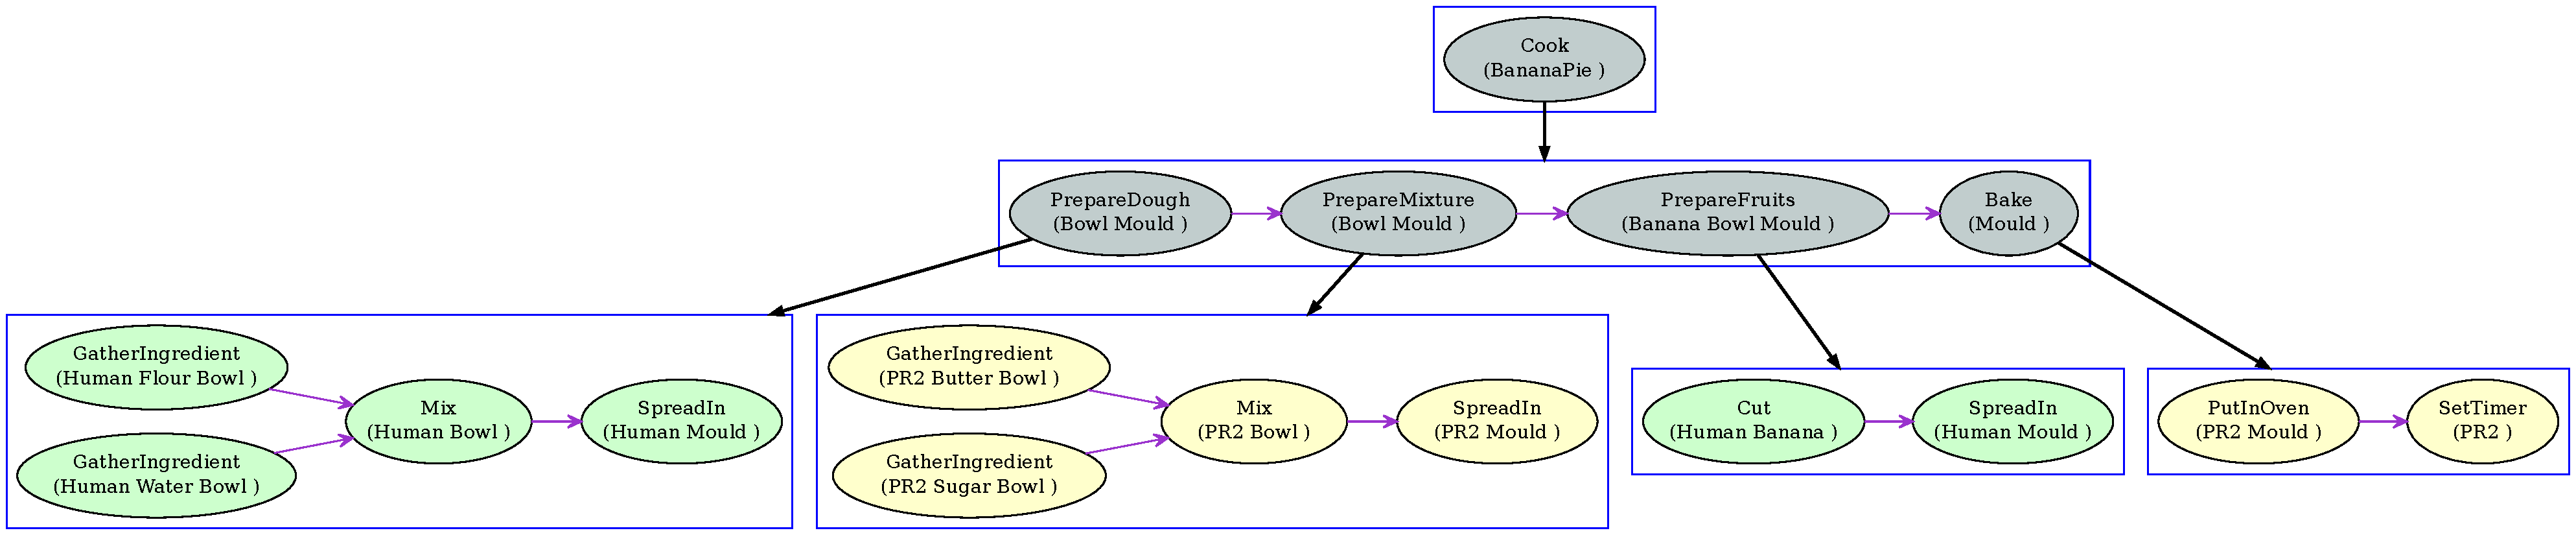
\includegraphics[width=0.99\textwidth]{img/plan_management/bananaPie.pdf}
 \end{tabular}
   \vspace{-8pt}
 \caption{Shared plan and associated HTN generated to collaboratively make a banana pie.}
 \label{fig:plan_management-bananaPlan}
   \vspace{-22pt}
 \end{figure*}
 

\begin{enumerate}
\item The human will prepare the dough, kneading it and putting it in the mould.
\item The robot will prepare a mixture with butter and sugar, putting the ingredients in the mould.
\item The human will then prepare the required fruits, cutting them and adding them to the mixture..
\item Then, the human will prepare the dough for the top of the pie.
\item Finally, the robot will bake the pie, by putting it into the oven and setting a timer.
\end{enumerate} 

After completing task 1, the human's knowledge on how to prepare the dough will be improved. Consequently, during the execution of task 4, the robot will ask the user if he needs help to prepare the second dough. We imagine he answers ``no". The robot does not explain the task  and the system will upgrade the human's knowledge level for the \textit{PrepareDough} task to  \textit{intermediate}, after he completes. The human's knowledge of task 3, \textit{PrepareFruit}, will be represented as \textit{$<$human1, PrepareFruits, [fruit], VALUE$>$}. We consider the parameter of this task as \textit{class-link} , since the process will be the same for any fruit (cutting and putting in the mould). This way we use, as parameter, the class \textit{fruit} instead of the actual instances used in the task, \textit{apple} or \textit{banana}.

After cooking the first pie, the robot generates a plan to cook the banana pie. This time, we set the environment in order to allow  each agent to perform all the tasks. Preparing a banana pie is a similar process to the apple pie. The parameter will, of course, be differents, involving bananas and not apple. Also, the banana pie does not have a second dough on its top, and it has a different baking time from the apple pie. The plan generated is presented in figure \ref{fig:plan_management-bananaPlan}. We can observe that the planner took into account the experience acquired by the human when preparing the apple pie, by assigning him the tasks (\textit{PrepareDough} and \textit{PrepareFruits}). During execution, since the user has an \textit{intermediate} knowledge level on \textit{PrepareDough}, the robot will not explain it. When the human is about to execute \textit{PrepareFruits}, the robot will propose to explain him the task, since he only performed it once, and has a \textit{beginner} knowledge level on it.


\subsection{User Study}
We have conducted a comparative user study in order to have a first evaluation of our system's adaptability by users. Two groups of users were asked to participate in the two-pies scenario. The first group interacted with a simulated robot equipped with a basic system (BS). BS has the same behavior as our system, excluding the agent knowledge awareness mechanisms. The second group interacted with another system, which we will refer to as knowledge system (KS), and exhibits similar characterstics to the presented system.

The hypothesis of our study is that, on average, users will express a preference on KS over BS. More formally, we set our null $H_0$ and alternative $H_A$ hypotheses as follows:
\begin{itemize}
\item $H_0$: $\mu_{KS}-\mu_{BS}==0$ 
\item $H_A$: $\mu_{KS}-\mu_{BS}!=0$  
\end{itemize}


In both system, we will use the same task allocation presented in subsection \ref{sec:plan_management-experiment} to achieve the apple pie cooking example. Once the have cooked the first dessert, the robot generates a plan to cook the banana pie. 
In KS,  the robot favors a task distribution for the banana pie where the human performs tasks he has already executed in the previous scenario (preparing dough and fruits).
In BS, we imagine that the robot could allocate the tasks differently, asking the human to prepare the mixture instead of the dough.

Two groups of 19 participants, from 18 to 60, interacted with each system in an online user study\footnote{User study for KS http://goo.gl/forms/qvbtu4vcFW, and BS http://goo.gl/forms/ZSvGcCi5le}, where we presented pictures of the task state and recordings of the robot's speech, in French, for each step of the interaction (as shown in figure~\ref{fig:plan_management-user_study}).
At some steps, the user could choose the action to perform, allowing him to execute a wrong action, leading to a replan from the robot. For simplicity, the replan just corrected the wrong action, before resuming the previous plan. Also, since the focus of this study is only on the capacity of our system to adapt to users' knowledge, we did not allow a negotiation process.
At the end of the simulated interaction, we have asked the same questions to both groups, concerning the adaptability of the system and the robot partner itself. 
The users gave marks along a Likert scale from one (disagree) to five (agree) to express their agreement with several statements (as shown in figure \ref{fig:plan_management-user_study}).

\begin{figure}[ht!]
 \centering
 \begin{tabular}{cc}
  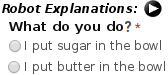
\includegraphics[width=0.24\textwidth]{img/plan_management/ustudy9.png} &
  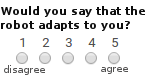
\includegraphics[width=0.19\textwidth]{img/plan_management/ustudy11.png}
 \end{tabular} 
 \caption[User studies on plan adaptation]{\textit{Left}: The user listens to recorded robot explanation and chooses the action to take. \textit{Right}: At the end, the user evaluates the interaction using a Likert scale.}
 \label{fig:plan_management-user_study}
 \end{figure}

\subsection{Results}

We collected the answers from each form, and computed the mean, along with the standard deviation and p-value to evaluate the system. The p-value was computed using a t-distribution with 18 degrees of freedom and evaluated using a significance value $\alpha=0.05$.
%We compare below the results for each system. 
Figure~\ref{fig:plan_management-results} summarizes the results. Comparing users' answers, we can see that user appreciated the capacity of the system to explain the plan while  adaptation on their knowledge, with a mean of 3.74 for KS against 2.05 for BS. The users interacting with KS globally noticed that the task distribution took their knowledge into account, by giving a mean rating of 3.42 for KS and 2.58 for BS. The last question concerned the freedom to choose how to perform the task. In this case, the calculated mean was 2.58 for KS and 1.89 for BS. In all these cases, the p-value was lower than the $\alpha$. 

With KS, the users attributed a mean of 3.11 for the global adaptability of the system against 1.89 for the basic one.
We also asked how the robot partner was perceived. While in KS the robot is not perceived as more verbose (2.53 for KS against 2.47 for BS), people found the interaction slightly more natural (2.74 against 2.42) and the robot appeared smarter (2.79 against 2.26). Even if these last two results look favorable, since their p-value is higher than $\alpha$  we do not have enough evidence to prove a difference between the two systems. We believe that other aspects might have been taken into account by the users, such as the speech itself, which conditioned their perception on the naturalness of the interaction. Improving the robot's verbalization process with a synonym dictionary could be a first step to get more significant results.



 \begin{figure}[ht!]
 \centering
 \begin{tabular}{cc}
  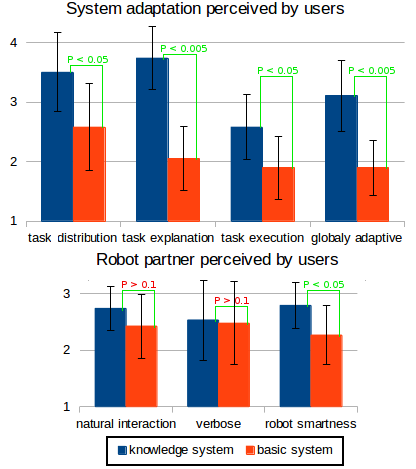
\includegraphics[width=0.45\textwidth]{img/plan_management/respvalue3.png}
 \end{tabular}
 \caption[Average users' rating of the interaction on several criteria]{Average users' rating of the interaction on several criteria. Blue for KS and red for BS.}
 \label{fig:plan_management-results}
 \end{figure}

This study sheds light on how users were able to perceive the robot adaptation to their knowledge concerning task distribution, task explanation and monitoring. In addition, the robot partner was perceived as smarter and the interaction seemed a bit more natural to the users. However, these first results need to be confirmed with study on a larger population. Also, as the scenario was simulated, results on a real robot might differ.
In both studies, we asked the participants how the system could be improved. Several users suggested they would like to be able to choose which action to perform, showing the importance of negotiation. A user suggested he would like to be informed about the progress of the task from time to time. Other comments concerned suggestions about the robot's speech capacities, like its voice voice, its intonation, and the chosen words. These aspects were not the aim of our  experiment but are indeed an important part of the interaction process. 

%


